\chapter{Results}

Combining the FLIP implementation described in chapter \ref{chapter flip impl} and the render algorithms in chapter \ref{chapter render}, the software of this project is able to generate realistic images of many interesting simulations in real time. Some selected sequences of screenshots follow below.



\begin{figure}[H]
    \centering
    
    \begin{minipage}[t]{.24\linewidth}
        \centering
        \vspace{0pt}
        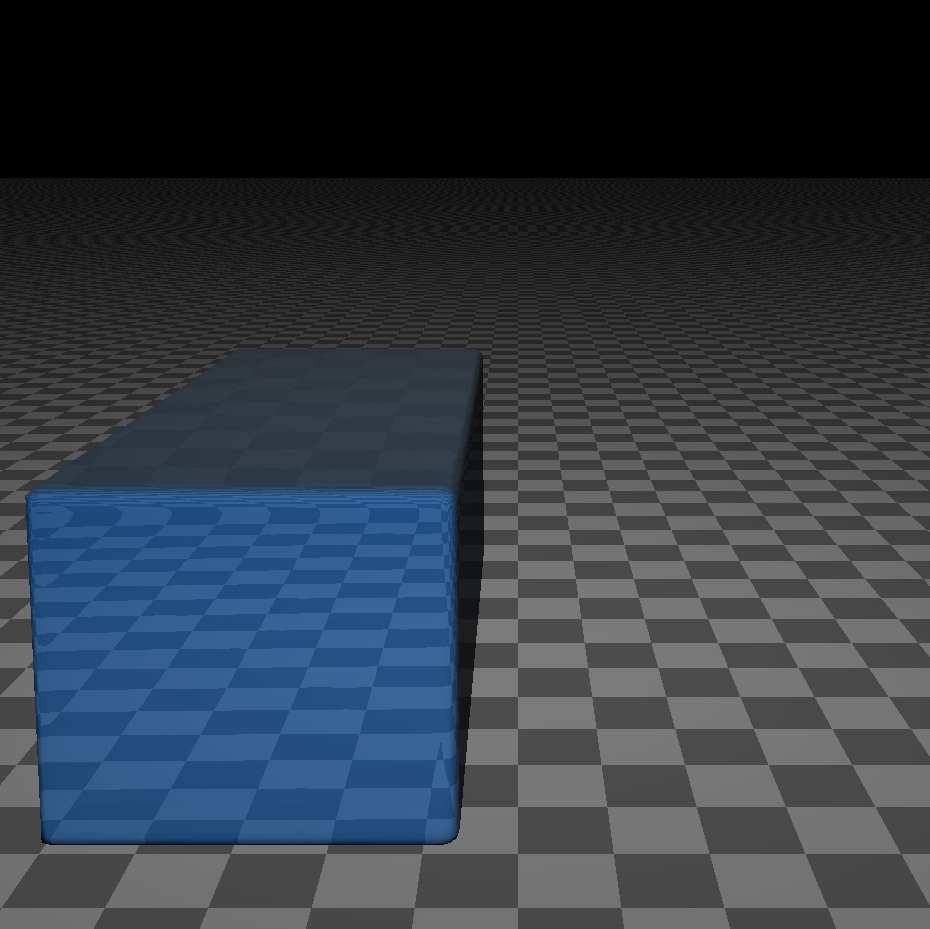
\includegraphics[width=3.5cm]{dambreak_cropped/0.png}
    \end{minipage}
    \begin{minipage}[t]{.24\linewidth}
        \centering
        \vspace{0pt}
        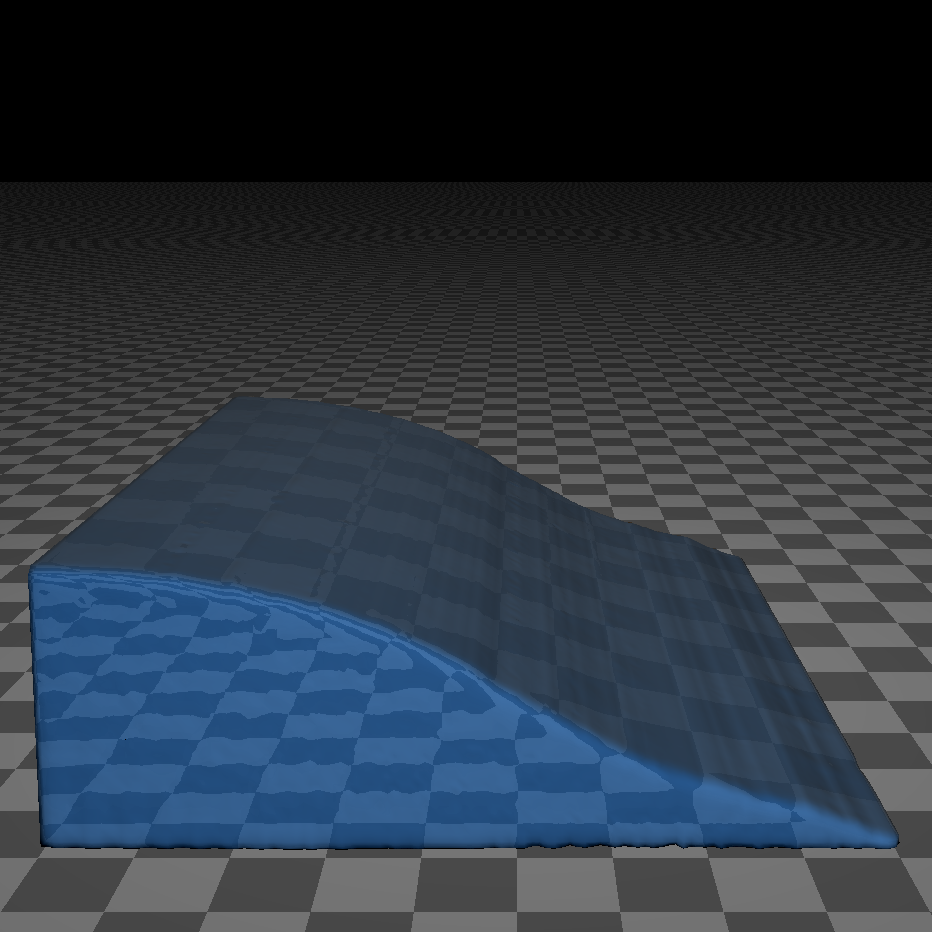
\includegraphics[width=3.5cm]{dambreak_cropped/1.png}
    \end{minipage}
    \begin{minipage}[t]{.24\linewidth}
        \centering
        \vspace{0pt}
        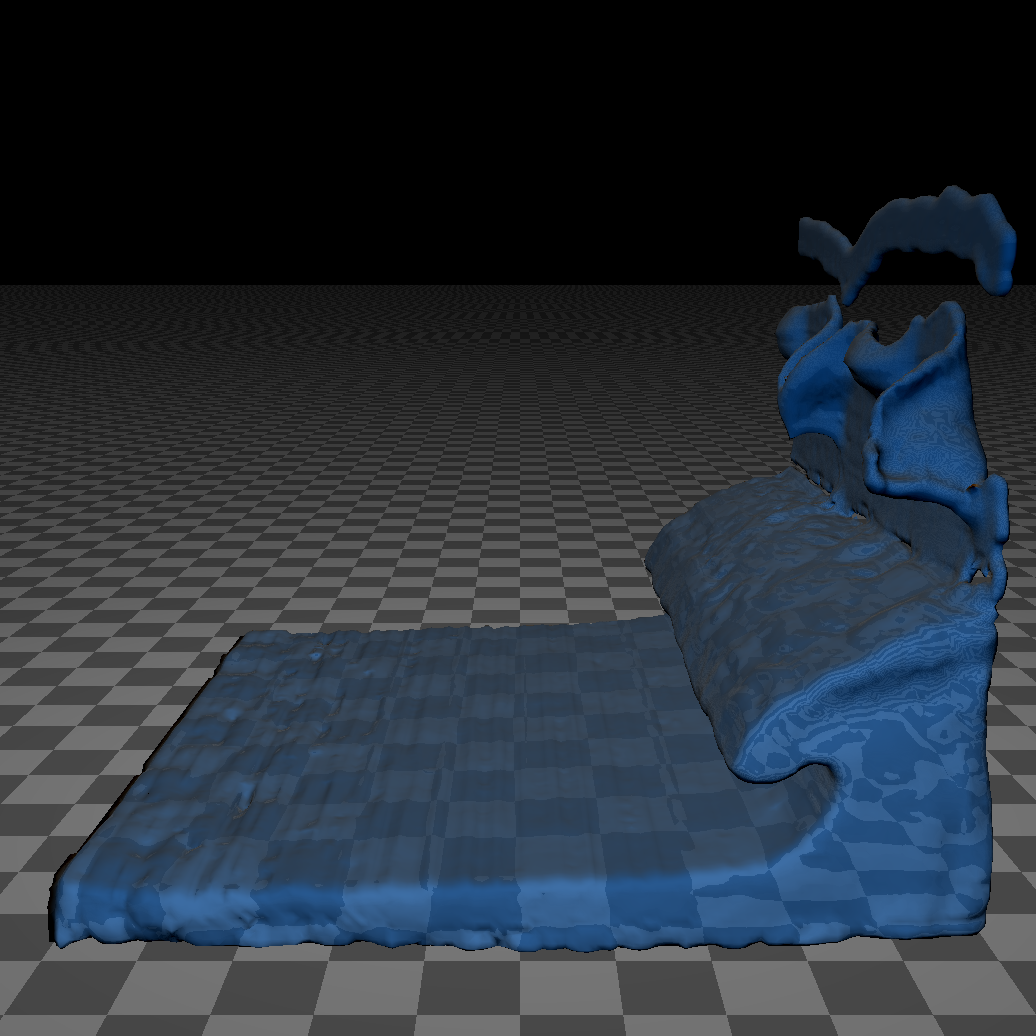
\includegraphics[width=3.5cm]{dambreak_cropped/2.png}
    \end{minipage}
    \begin{minipage}[t]{.24\linewidth}
        \centering
        \vspace{0pt}
        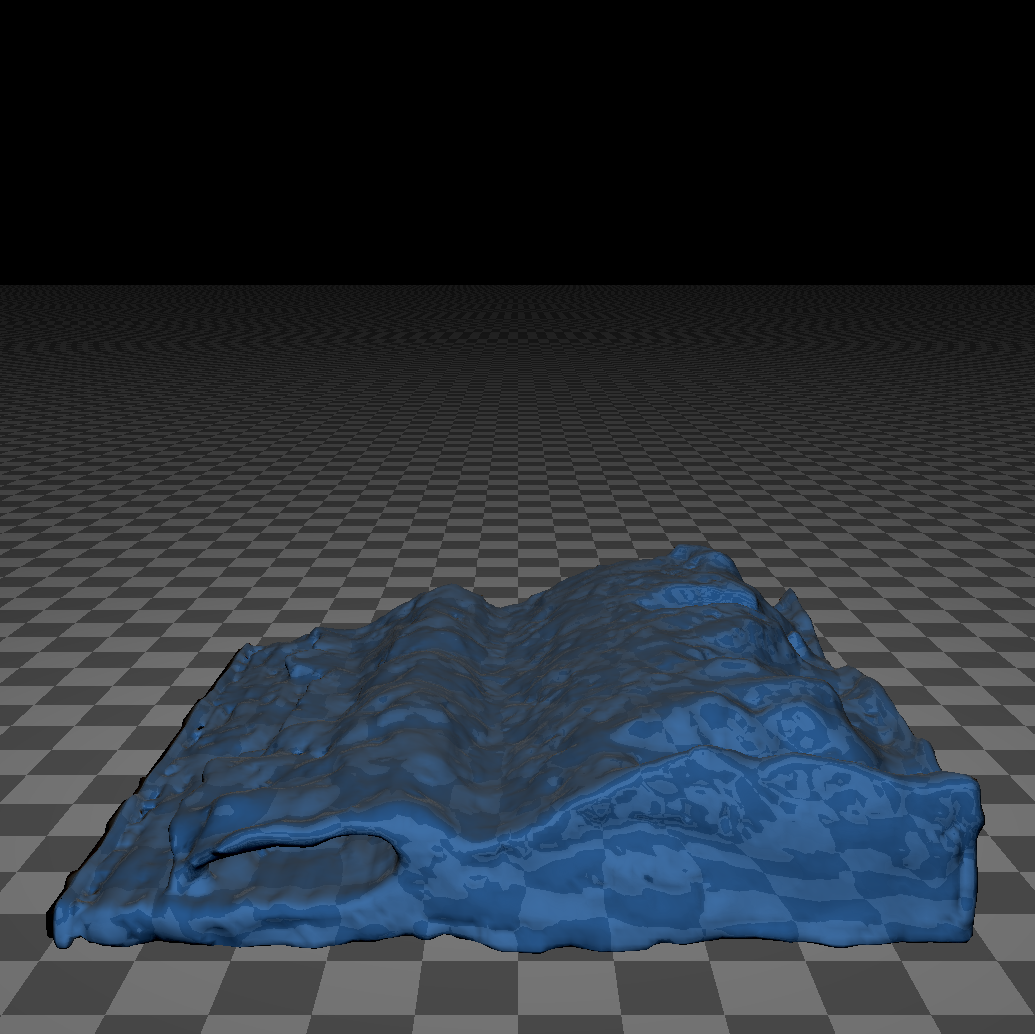
\includegraphics[width=3.5cm]{dambreak_cropped/3.png}
    \end{minipage}

    \caption{``Dam break" simulation}
    \label{fig dambreak}
\end{figure}

\begin{figure}[H]
    \centering
    
    \begin{minipage}[t]{.24\linewidth}
        \centering
        \vspace{0pt}
        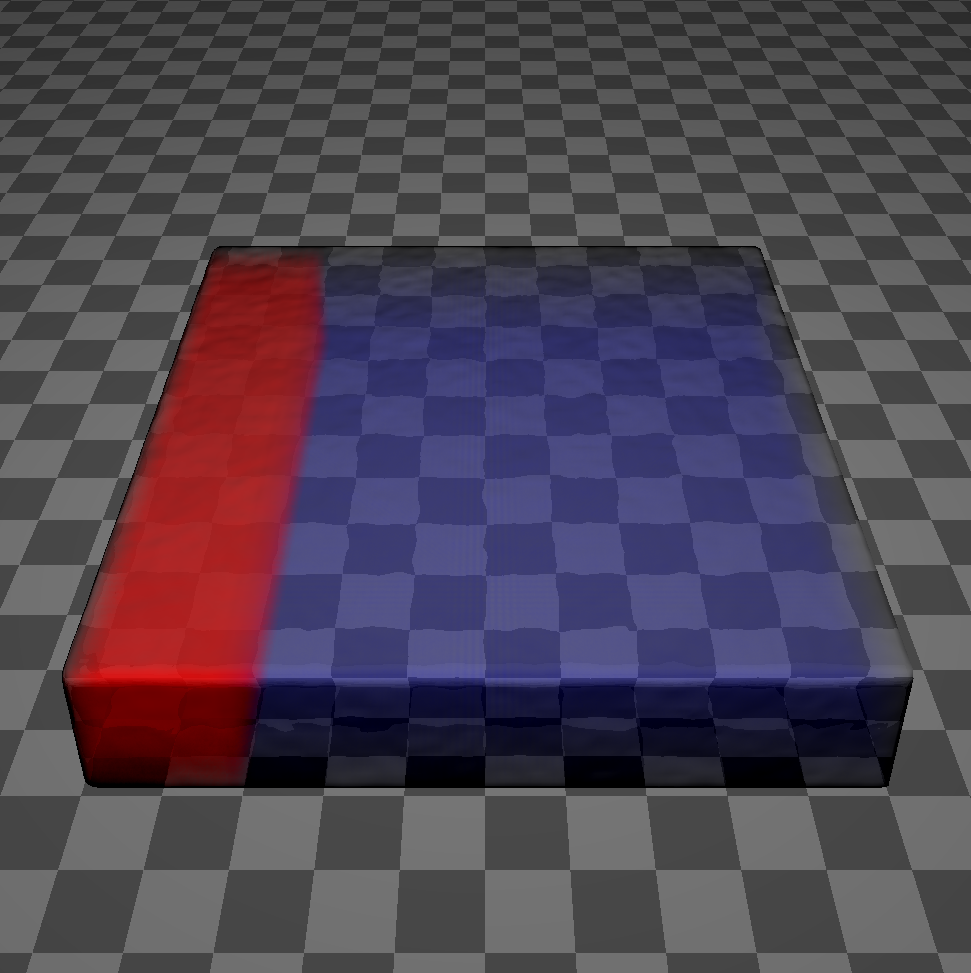
\includegraphics[width=3.5cm]{diffusion_cropped/small0.png}
    \end{minipage}
    \begin{minipage}[t]{.24\linewidth}
        \centering
        \vspace{0pt}
        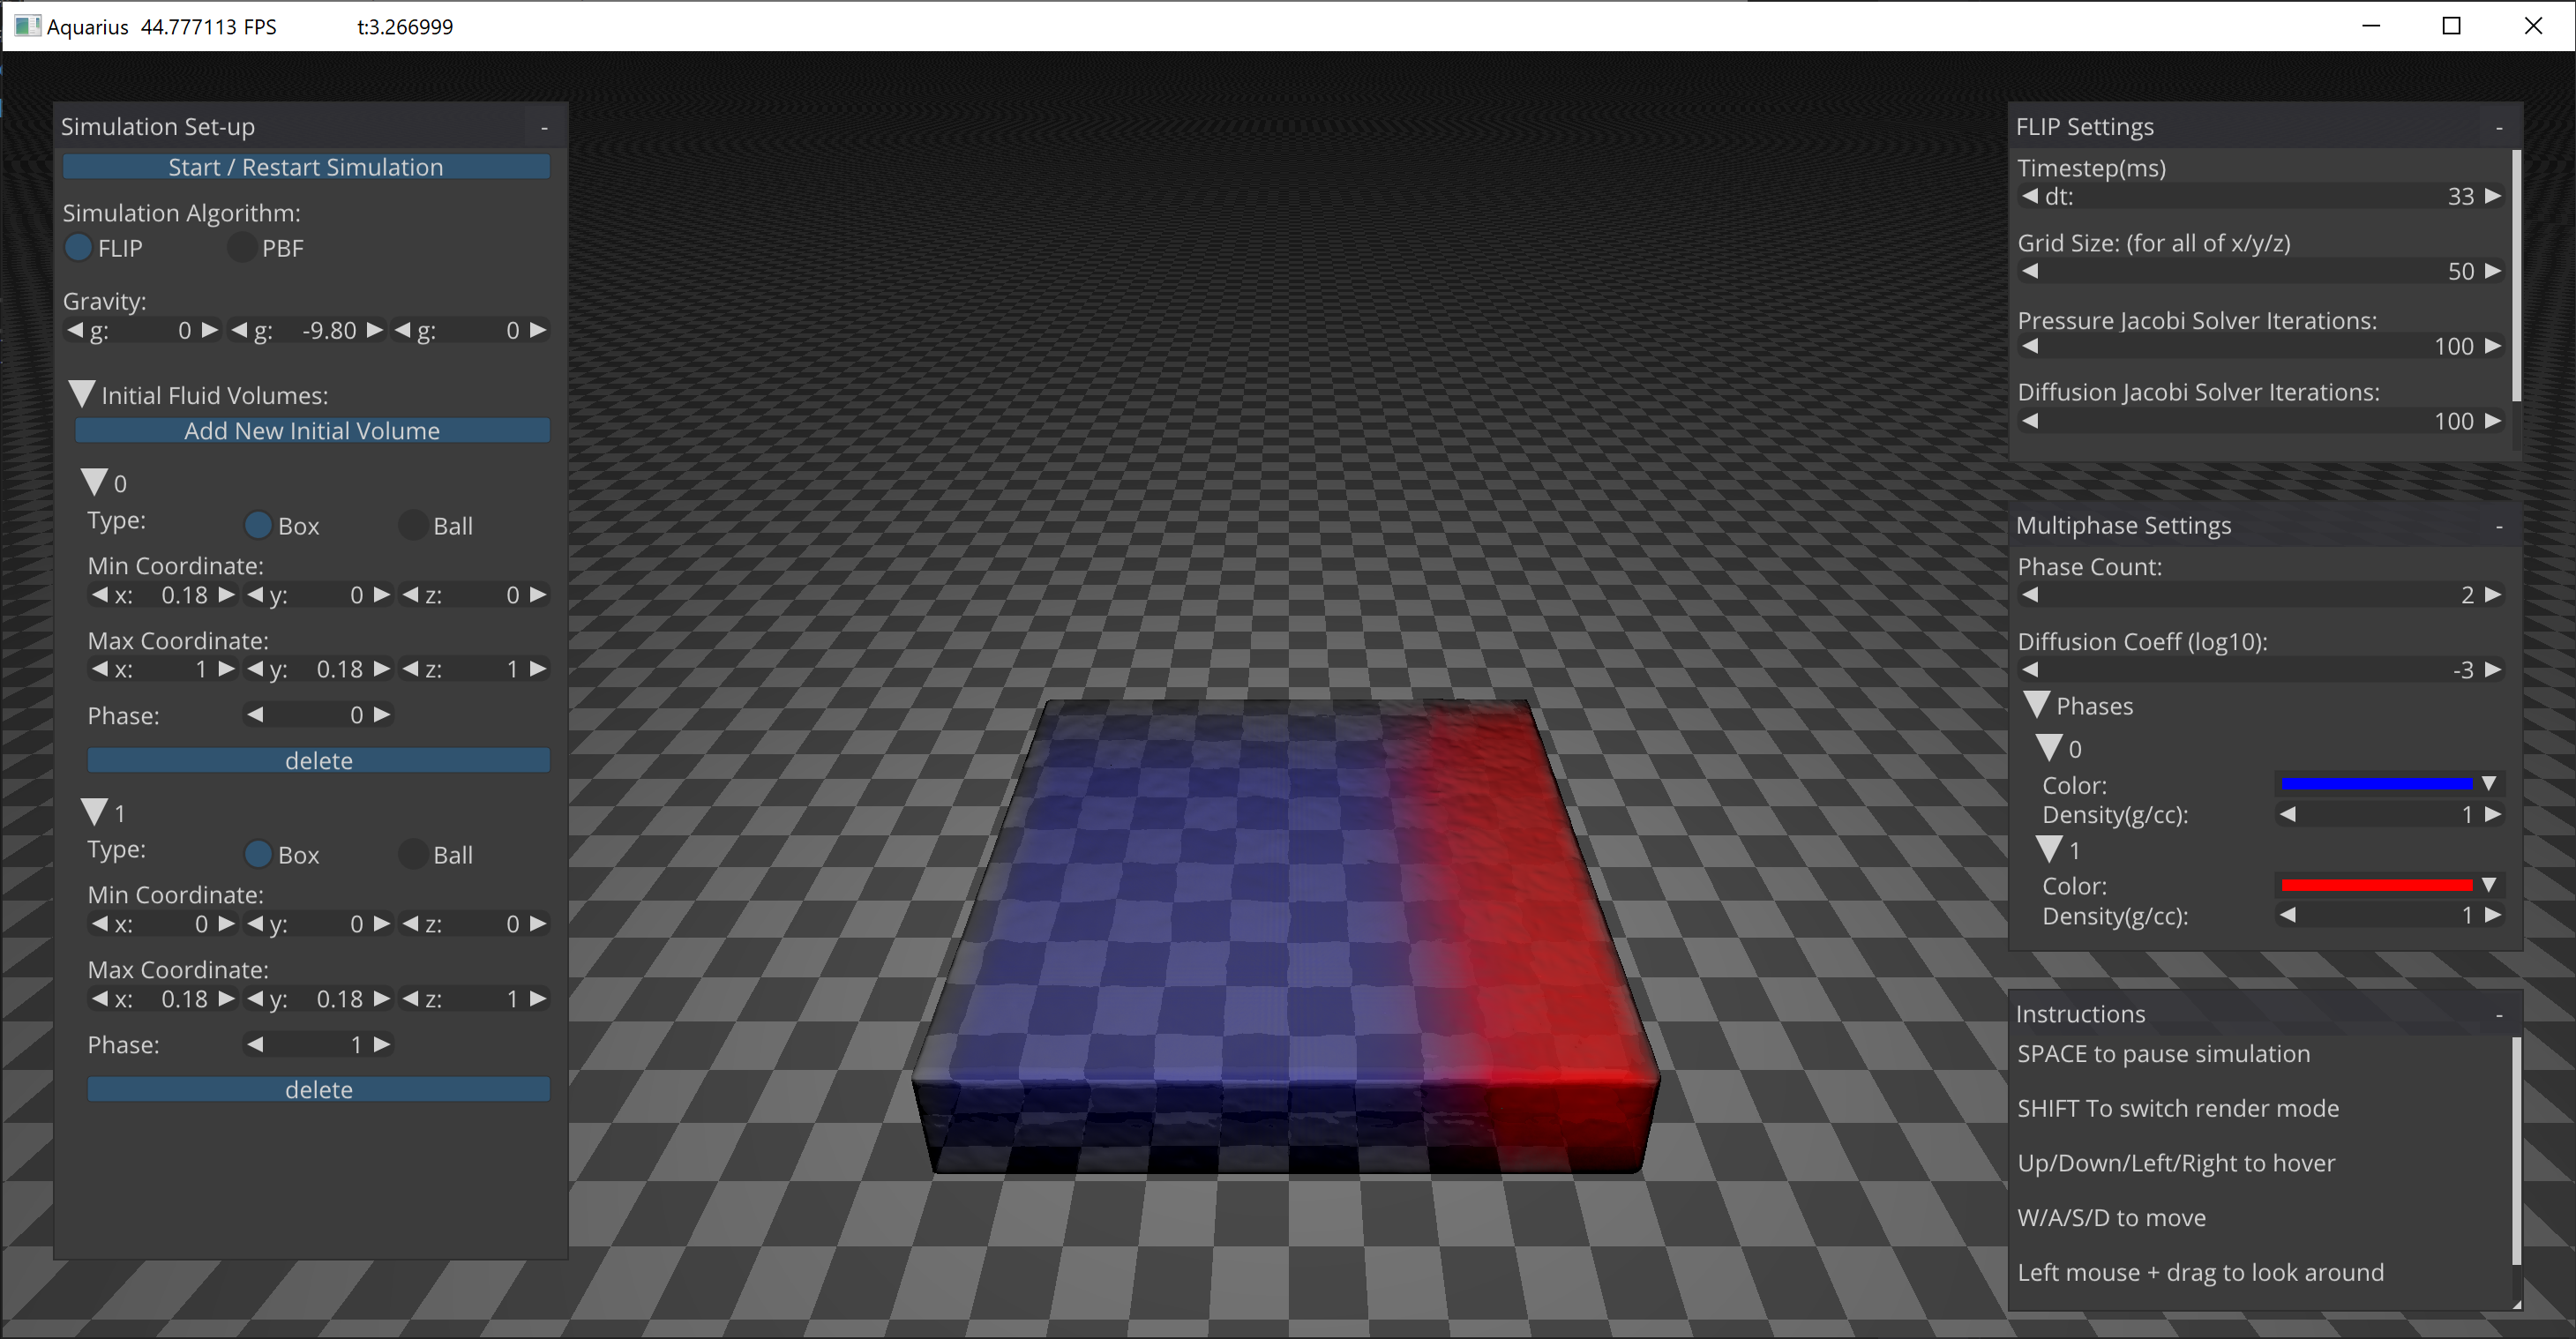
\includegraphics[width=3.5cm]{diffusion_cropped/small1.png}
    \end{minipage}
    \begin{minipage}[t]{.24\linewidth}
        \centering
        \vspace{0pt}
        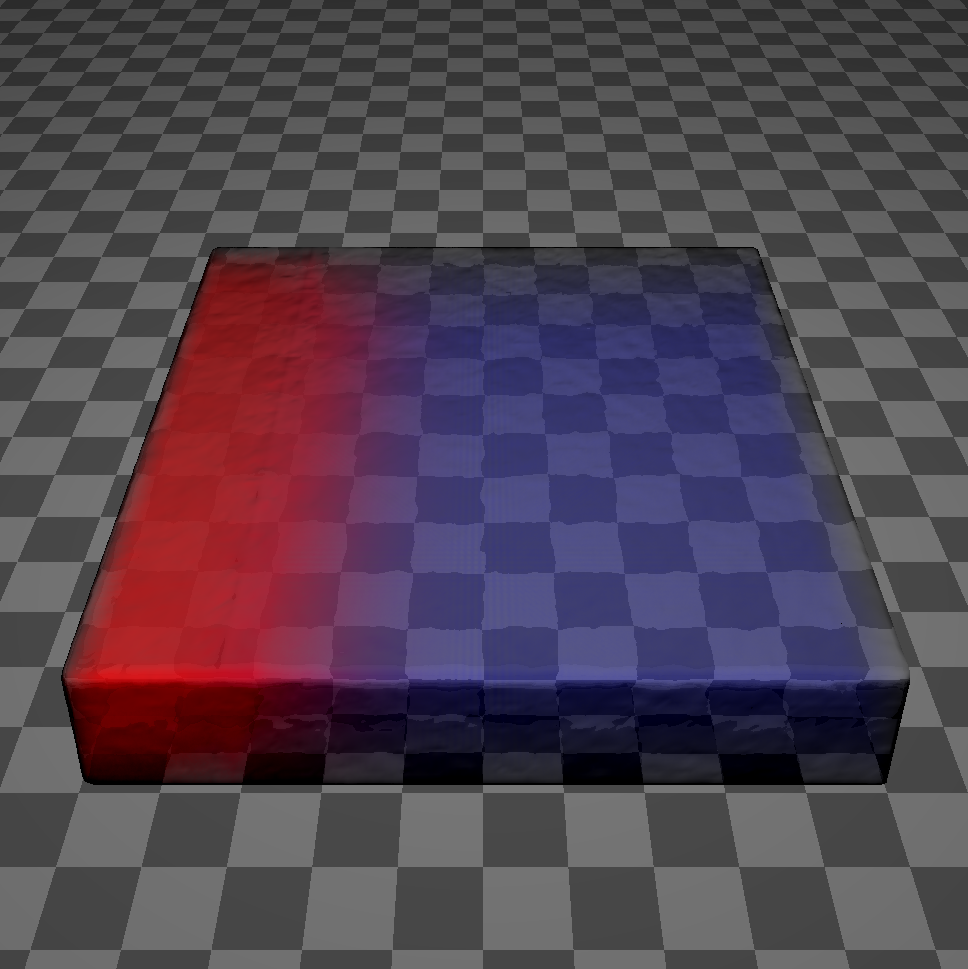
\includegraphics[width=3.5cm]{diffusion_cropped/small2.png}
    \end{minipage}
    \begin{minipage}[t]{.24\linewidth}
        \centering
        \vspace{0pt}
        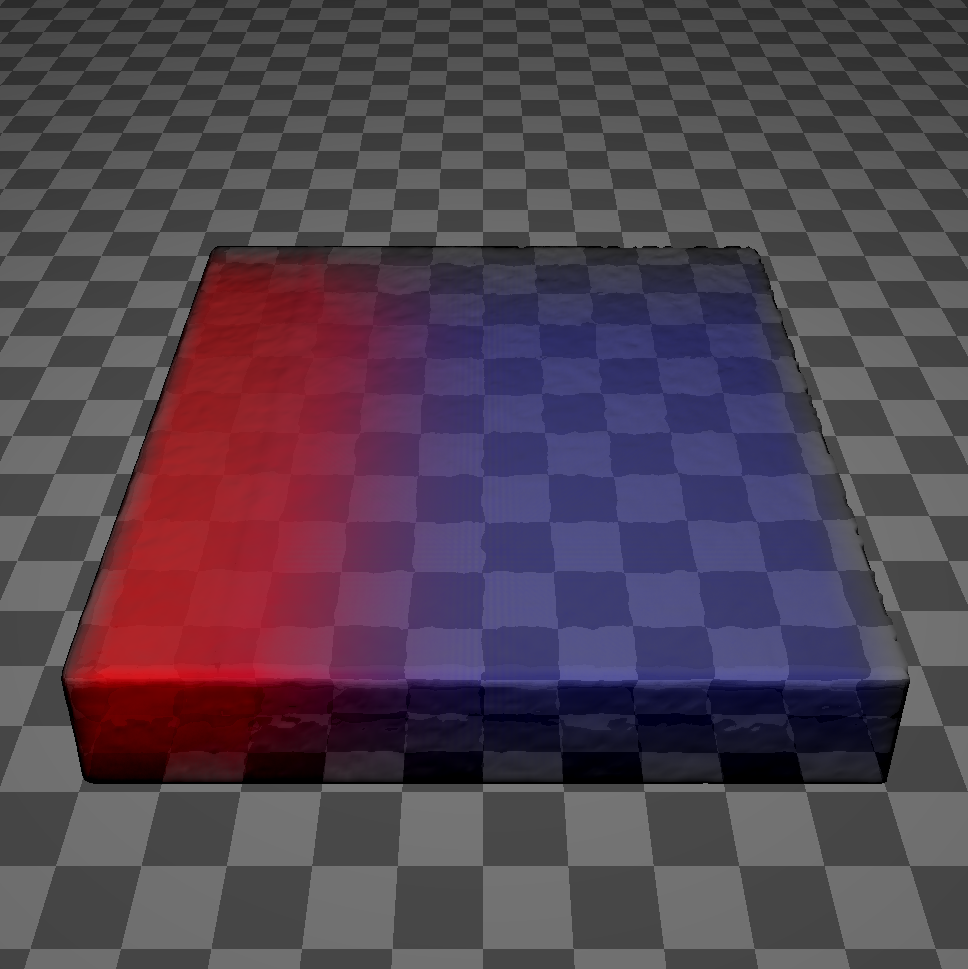
\includegraphics[width=3.5cm]{diffusion_cropped/small3.png}
    \end{minipage}

    \caption{Diffusion with coefficient $10^{-3}$}
    \label{fig diffusion 1e-3}
\end{figure}



\begin{figure}[H]
    \centering
    
    \begin{minipage}[t]{.24\linewidth}
        \centering
        \vspace{0pt}
        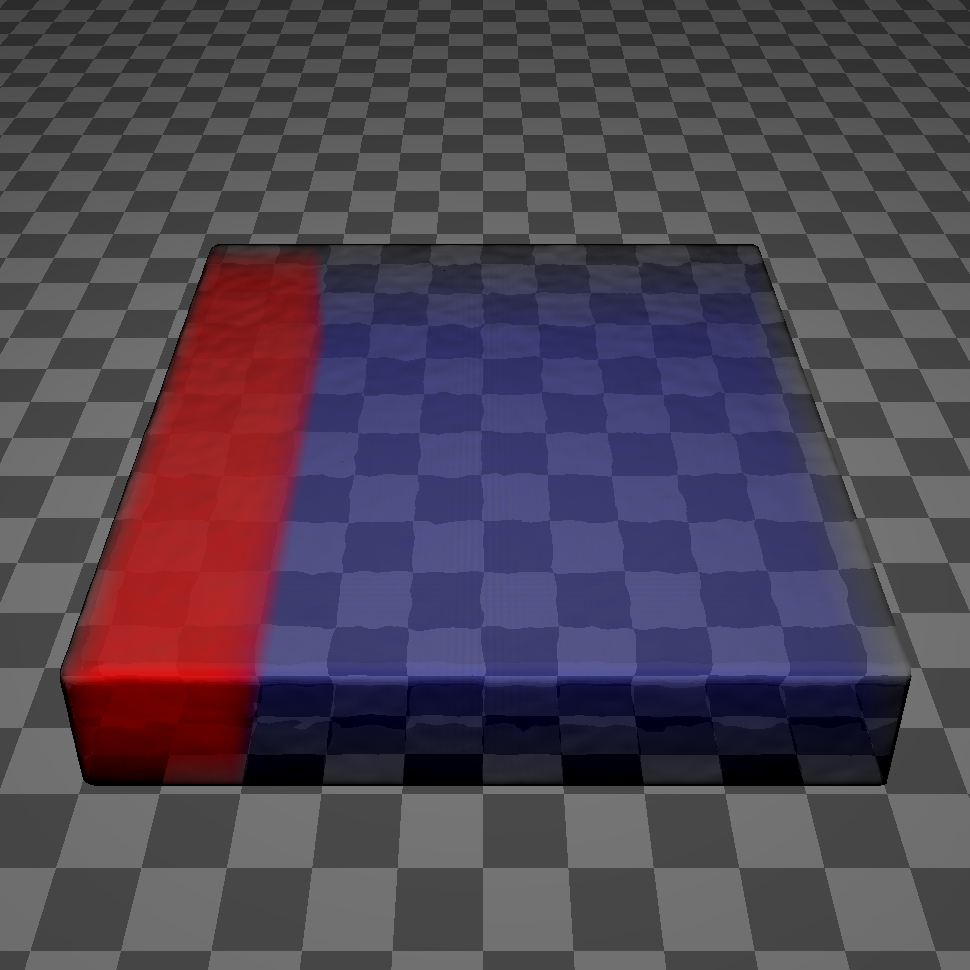
\includegraphics[width=3.5cm]{diffusion_cropped/big0.png}
    \end{minipage}
    \begin{minipage}[t]{.24\linewidth}
        \centering
        \vspace{0pt}
        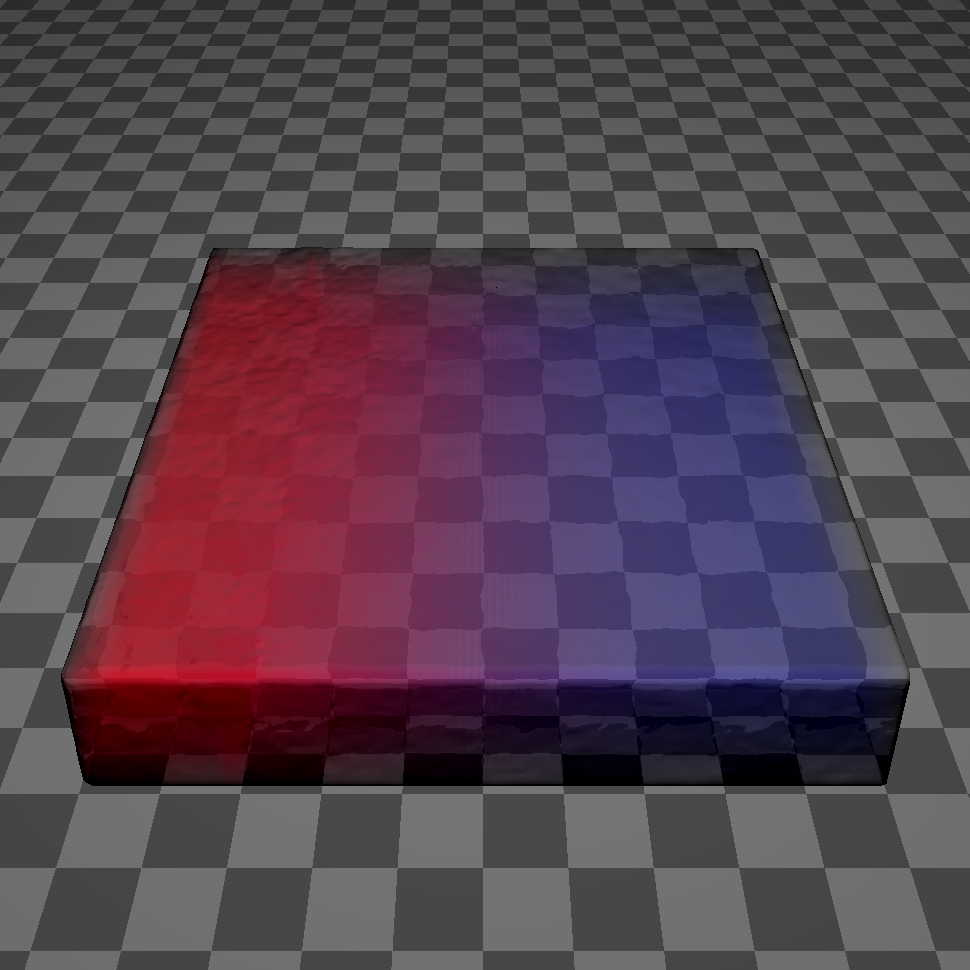
\includegraphics[width=3.5cm]{diffusion_cropped/big1.png}
    \end{minipage}
    \begin{minipage}[t]{.24\linewidth}
        \centering
        \vspace{0pt}
        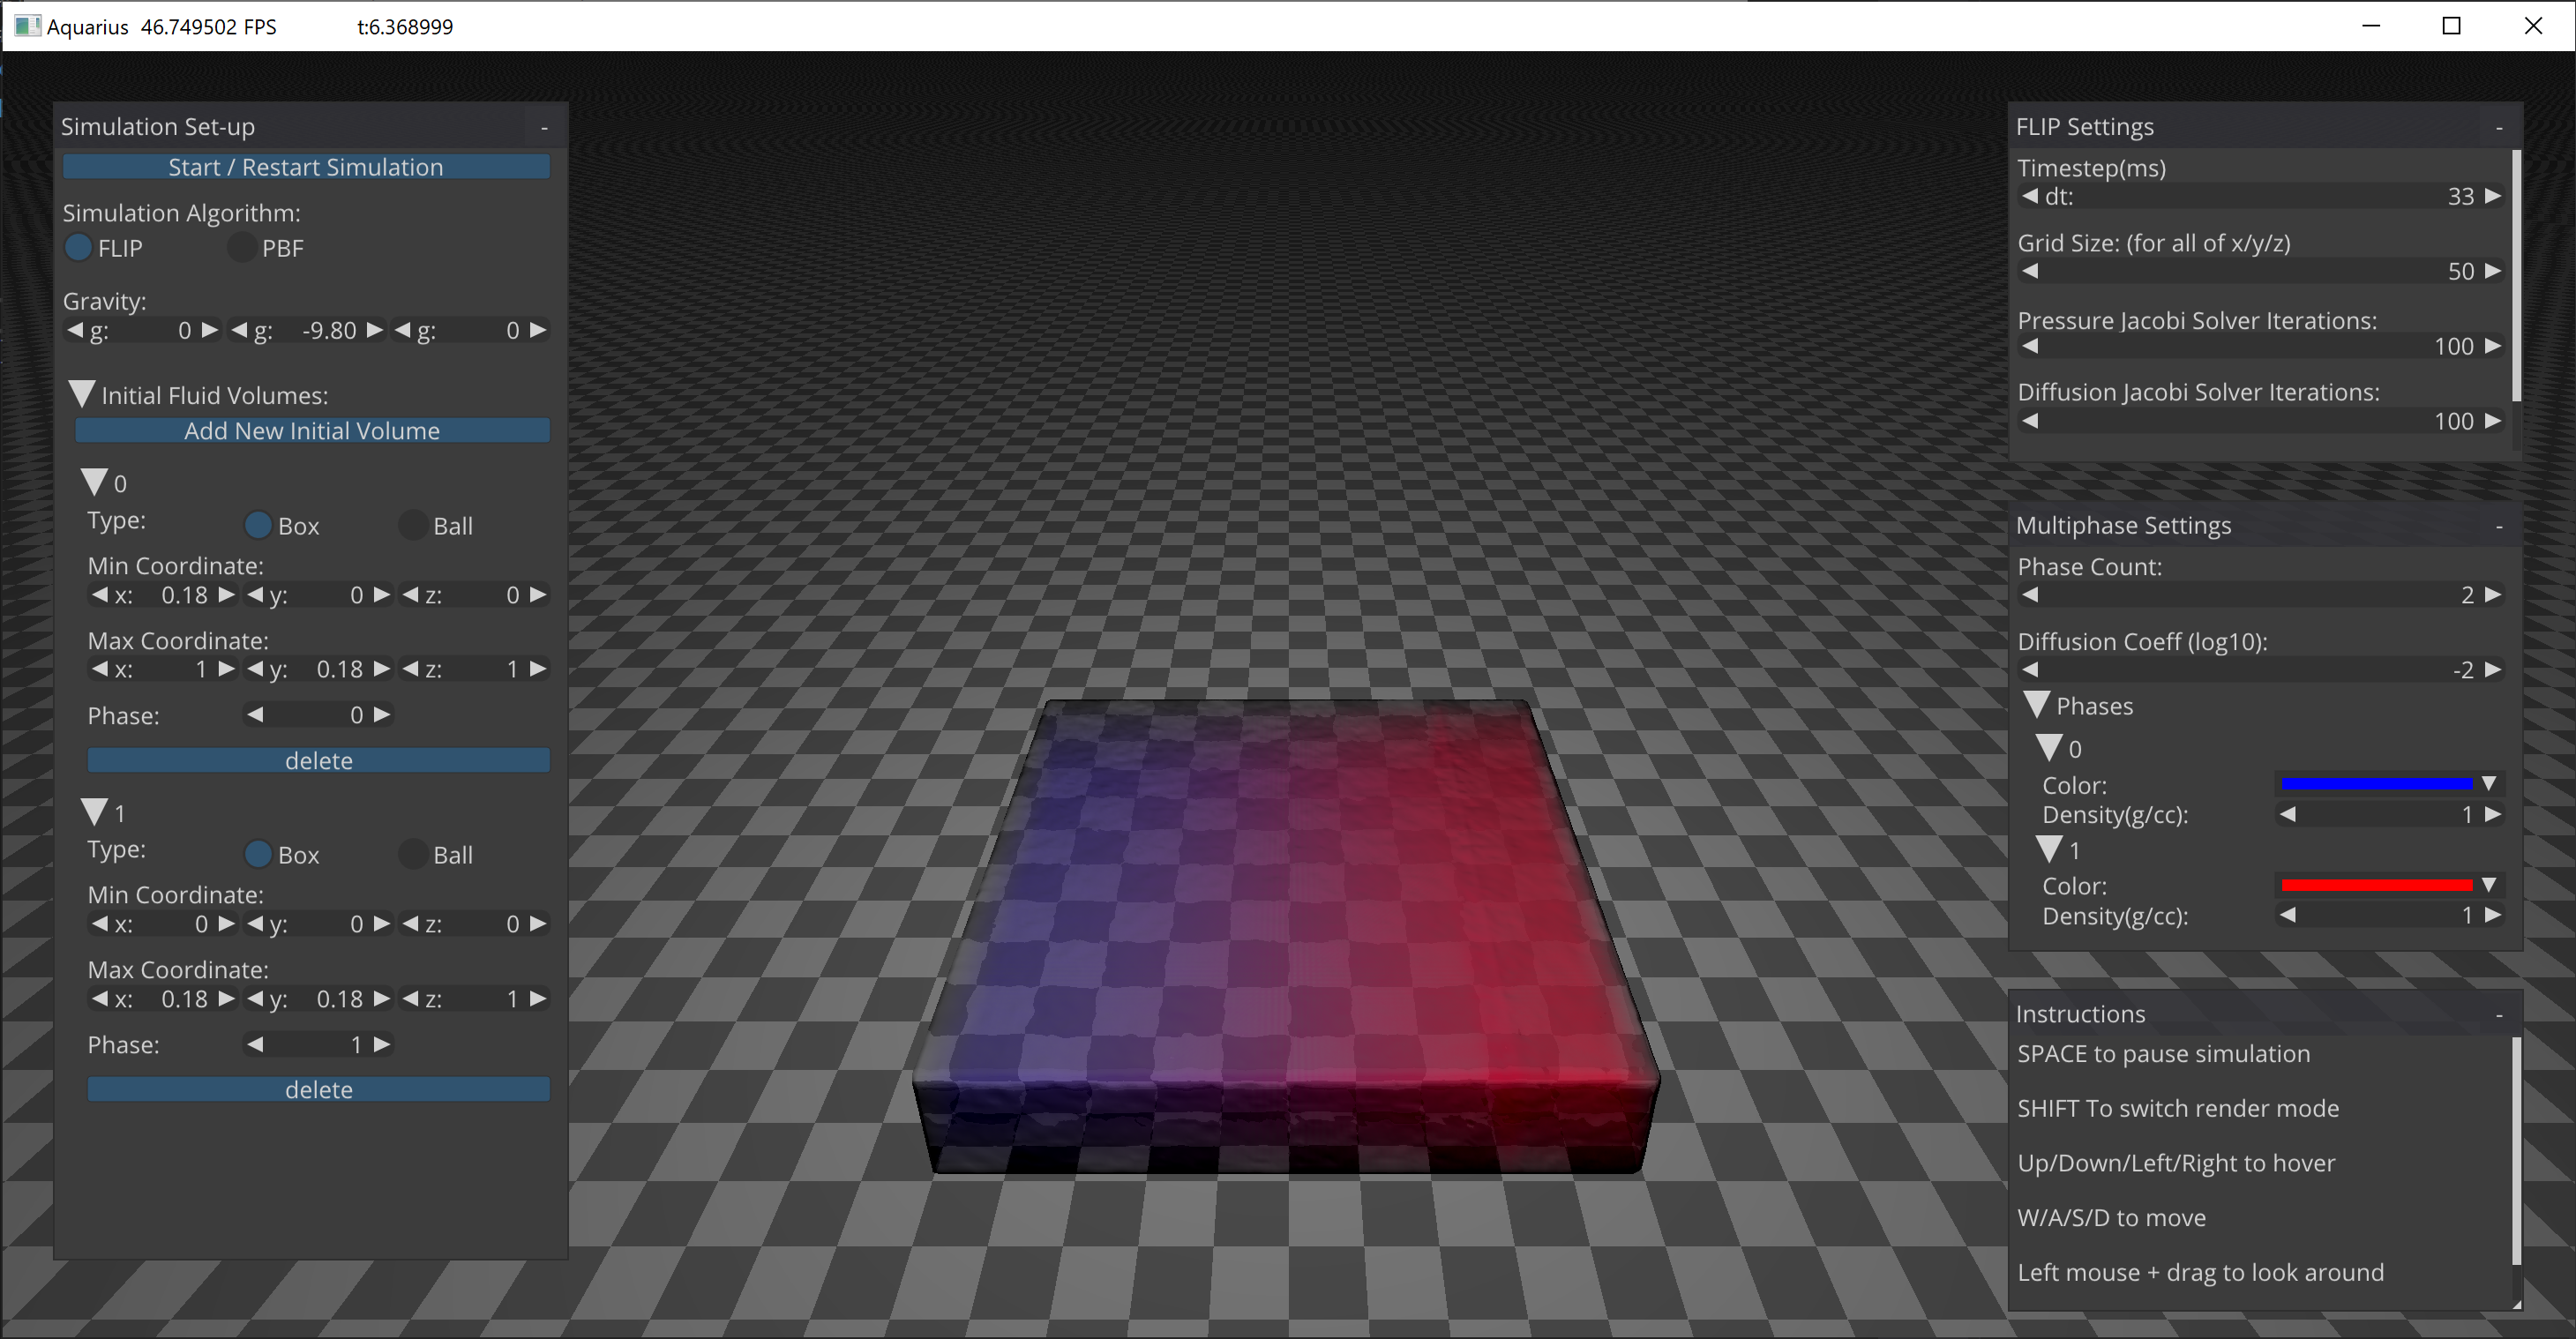
\includegraphics[width=3.5cm]{diffusion_cropped/big2.png}
    \end{minipage}
    \begin{minipage}[t]{.24\linewidth}
        \centering
        \vspace{0pt}
        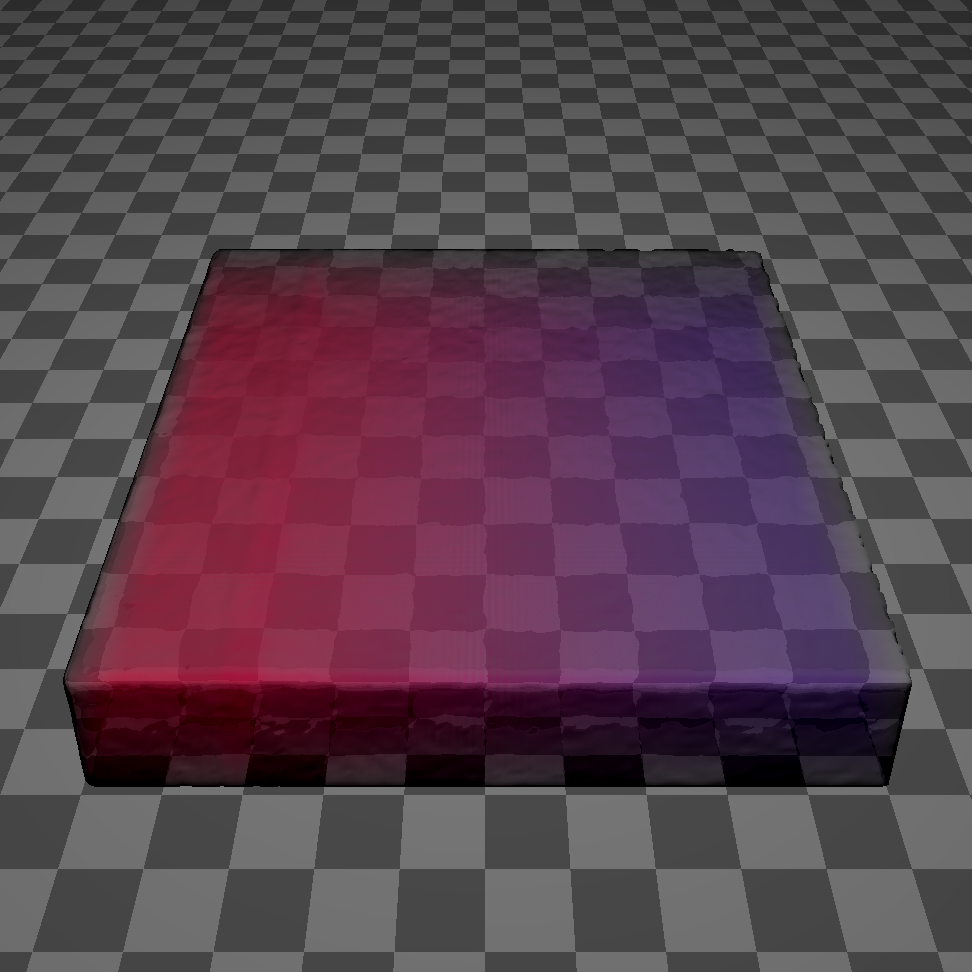
\includegraphics[width=3.5cm]{diffusion_cropped/big3.png}
    \end{minipage}

    \caption{Diffusion with coefficient $10^{-2}$}
    \label{fig diffusion 1e-2}
\end{figure}

\section{Performances}

Performances of the software implemented in this project highly depend on the simulation parameters used. The most influential parameter is the grid resolution, which is required to be at least approximately $50^3$ to give pleasing visual results. The simulation and rendering algorithms take time linear to the number of cells occupied by fluids, which is cubic to the grid resolution in each dimension. In the following figure, the empirical framerate of the software is plotted against the resolution:

\begin{figure}[H]
    \centering

    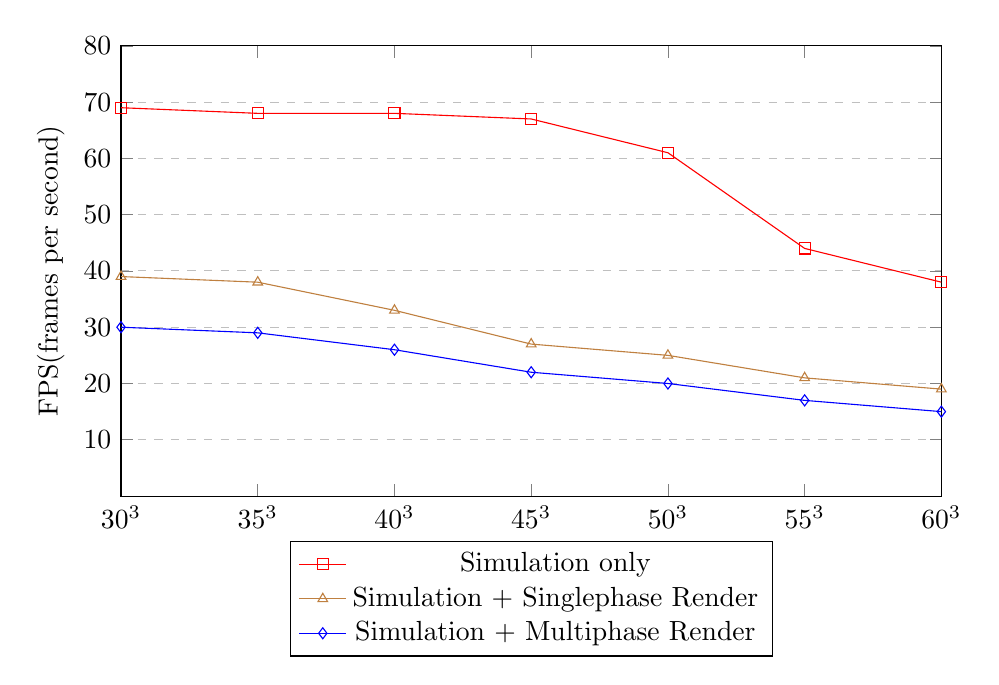
\begin{tikzpicture}
        \begin{axis}[
            xlabel={Grid resolution},
            ylabel={FPS(frames per second)},
            xmin=30, xmax=60,
            ymin=0, ymax=80,
            xtick={30,35,40,45,50,55,60},
            ytick={10,20,30,40,50,60,70,80},
            xticklabels={$30^3$,$35^3$,$40^3$,$45^3$,$50^3$,$55^3$,$60^3$},
            ymajorgrids=true,
            grid style=dashed,
            width=12cm,height=7.3cm,
            legend style={at={(0.5,-0.1)},anchor=north}
        ]
        
        \addplot[
            color=red,
            mark=square,
            ]
            coordinates {
            (30,69)(35,68)(40,68)(45,67)(50,61)(55,44)(60,38)
            };
            \addlegendentry{Simulation only}
        
        \addplot[
            color=brown,
            mark=triangle,
            ]
            coordinates {
            (30,39)(35,38)(40,33)(45,27)(50,25)(55,21)(60,19)
            };
            \addlegendentry{Simulation + Singlephase Render}
        
        \addplot[
            color=blue,
            mark=diamond,
            ]
            coordinates {
            (30,30)(35,29)(40,26)(45,22)(50,20)(55,17)(60,15)
            };
            \addlegendentry{Simulation + Multiphase Render}
            
        \end{axis}
        \end{tikzpicture}
    
    \caption{Plot of framerate against grid resolution. Each simulation uses the identical initial condition, where 25\% of the domain is occupied with fluid. 100 Jacobi iterations are used in each time step. The tests are performed on a Microsoft Surface Book 2, with a i7-8650U CPU and a GTX 1060 GPU.}
    \label{fig FPS vs grid res}
\end{figure}


As a somewhat surprising observation, the computation time required to render a frame is actually considerable longer then the time taken to advance the simulation by one step. This is because, in order to generate a fine mesh, the resolution of the discrete grid of signed distance field is around 3 times the resolution of the MAC grid, which caused the surface reconstruction step (section \ref{section surface reconstruction}) to be rather expensive. Furthermore, multiphase rendering is noticeably more expensive then single phase rendering, which is because if there is only one fluid phase, the particle-based optical thickness calculation (section \ref{subsection multiphase render}) needs not be applied, and an approximation can be made using the tint color of the fluid.

\section{Comparison with Existing Software}

The performance of the software created in this project is compared with a public CPU implementation of FLIP, namely the FLIP Fluids add-on\footnote{\url{https://blendermarket.com/products/flipfluids}} to Blender\footnote{\url{https://www.blender.org/}}. The exact same simulation parameters are used, and the softwares are run on the same machine. Figure \ref{figure ball drop single}, \ref{figure ball drop multi}, and \ref{figure ball drop blender} shows an example comparison. In these figures, a $50^3$ grid is used, and while the CPU implementation in Blender takes around 1.1 seconds for each frame, the software of this project can perform simulation and rendering at $20$ FPS, which is substantially faster.

\gapM
\gapM
\gapM

\begin{figure}[H]
    \centering
    
    \begin{minipage}[t]{6.2cm}
        \centering
        \vspace{0pt}
        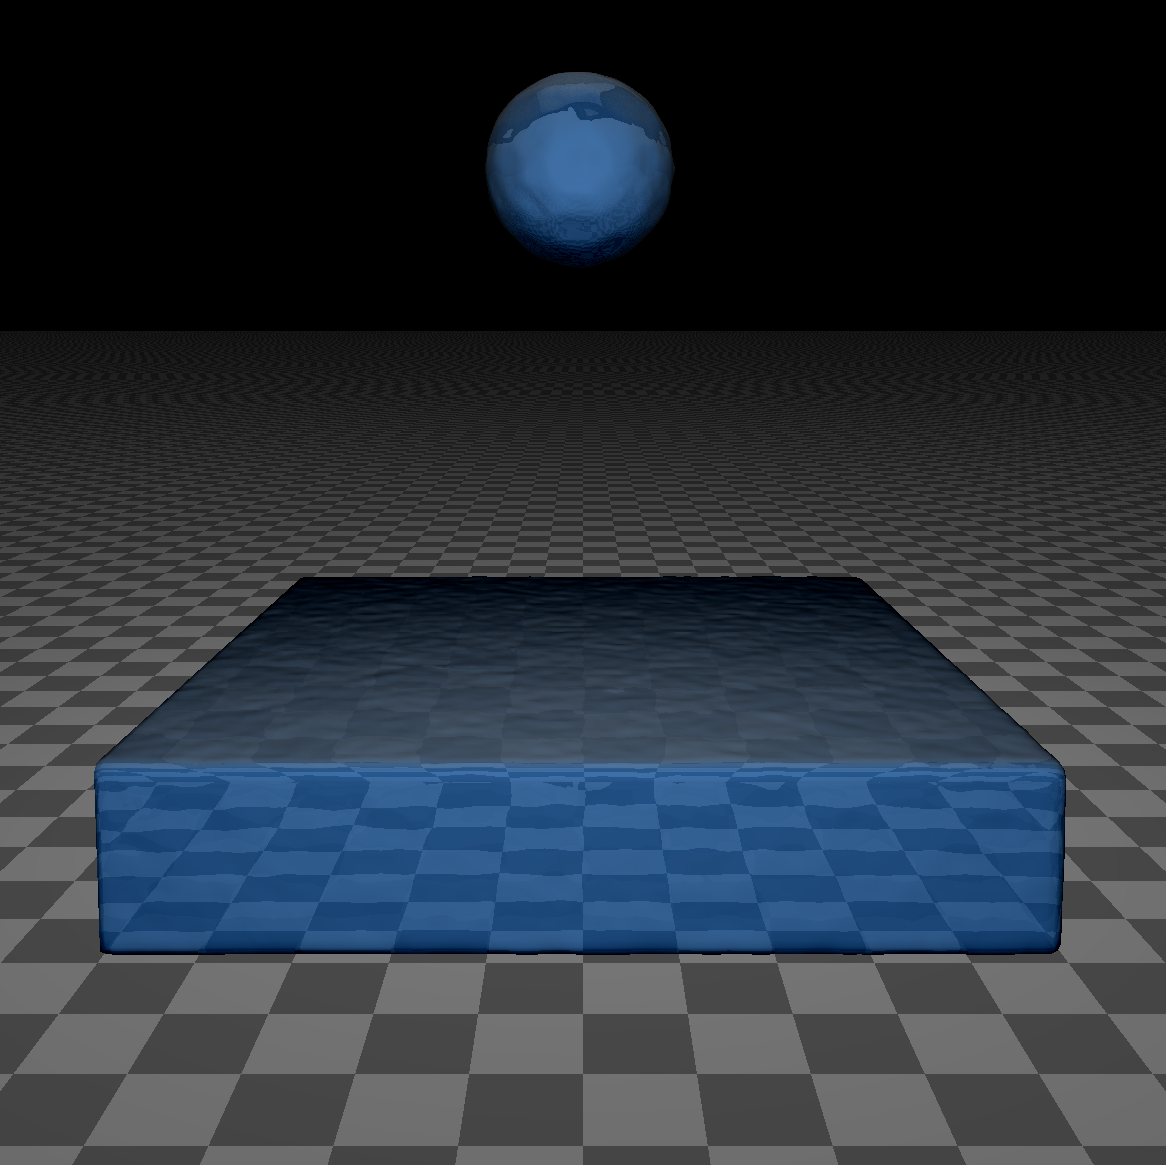
\includegraphics[width=5.7cm]{balldrop_cropped2/single0.png}
    \end{minipage}
    \begin{minipage}[t]{6.2cm}
        \centering
        \vspace{0pt}
        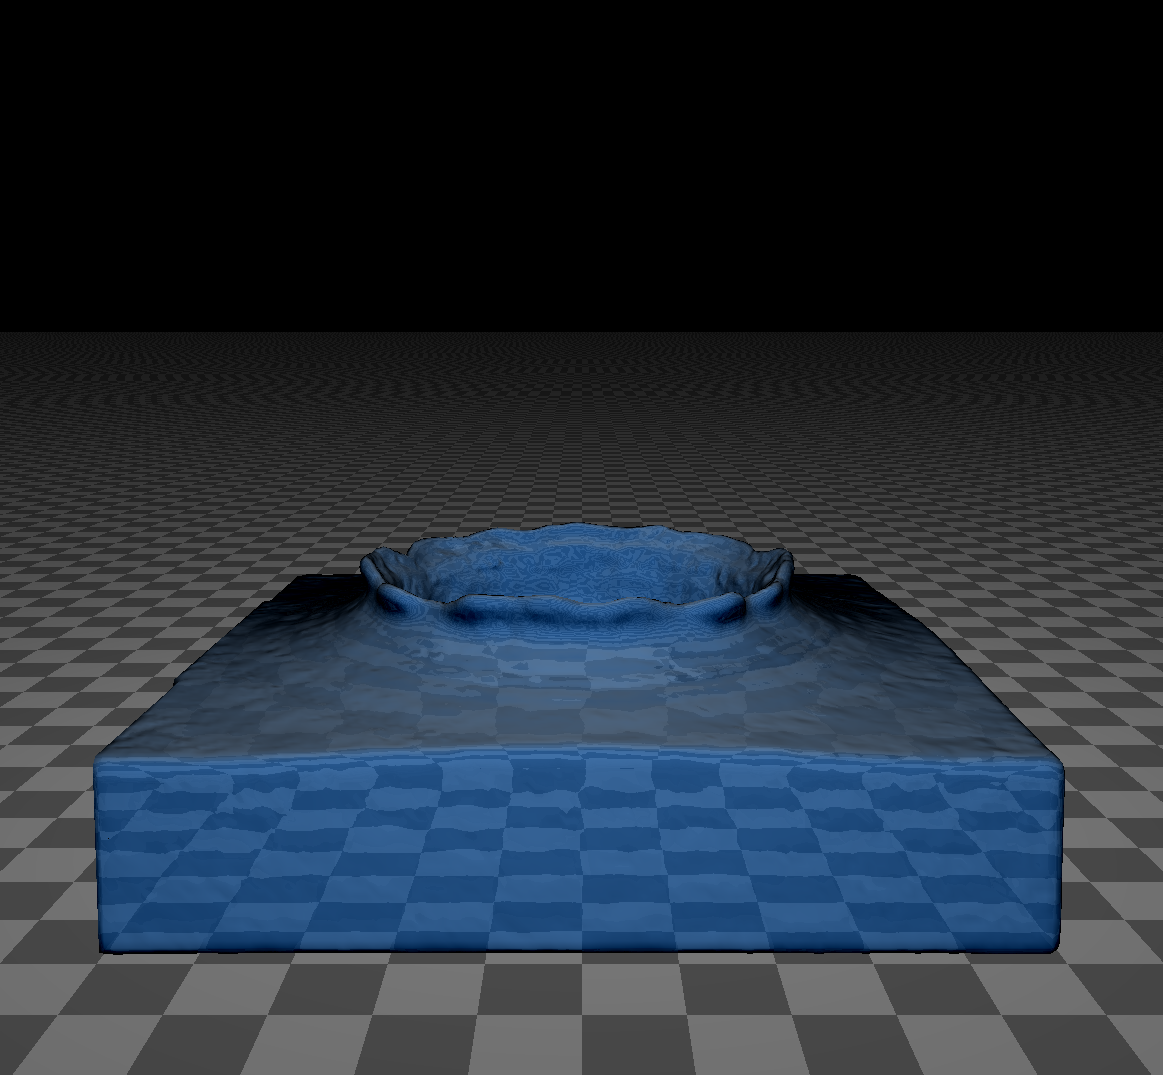
\includegraphics[width=5.7cm]{balldrop_cropped2/single1.png}
    \end{minipage}

    \vspace{0.5cm}

    \begin{minipage}[t]{6.2cm}
        \centering
        \vspace{0pt}
        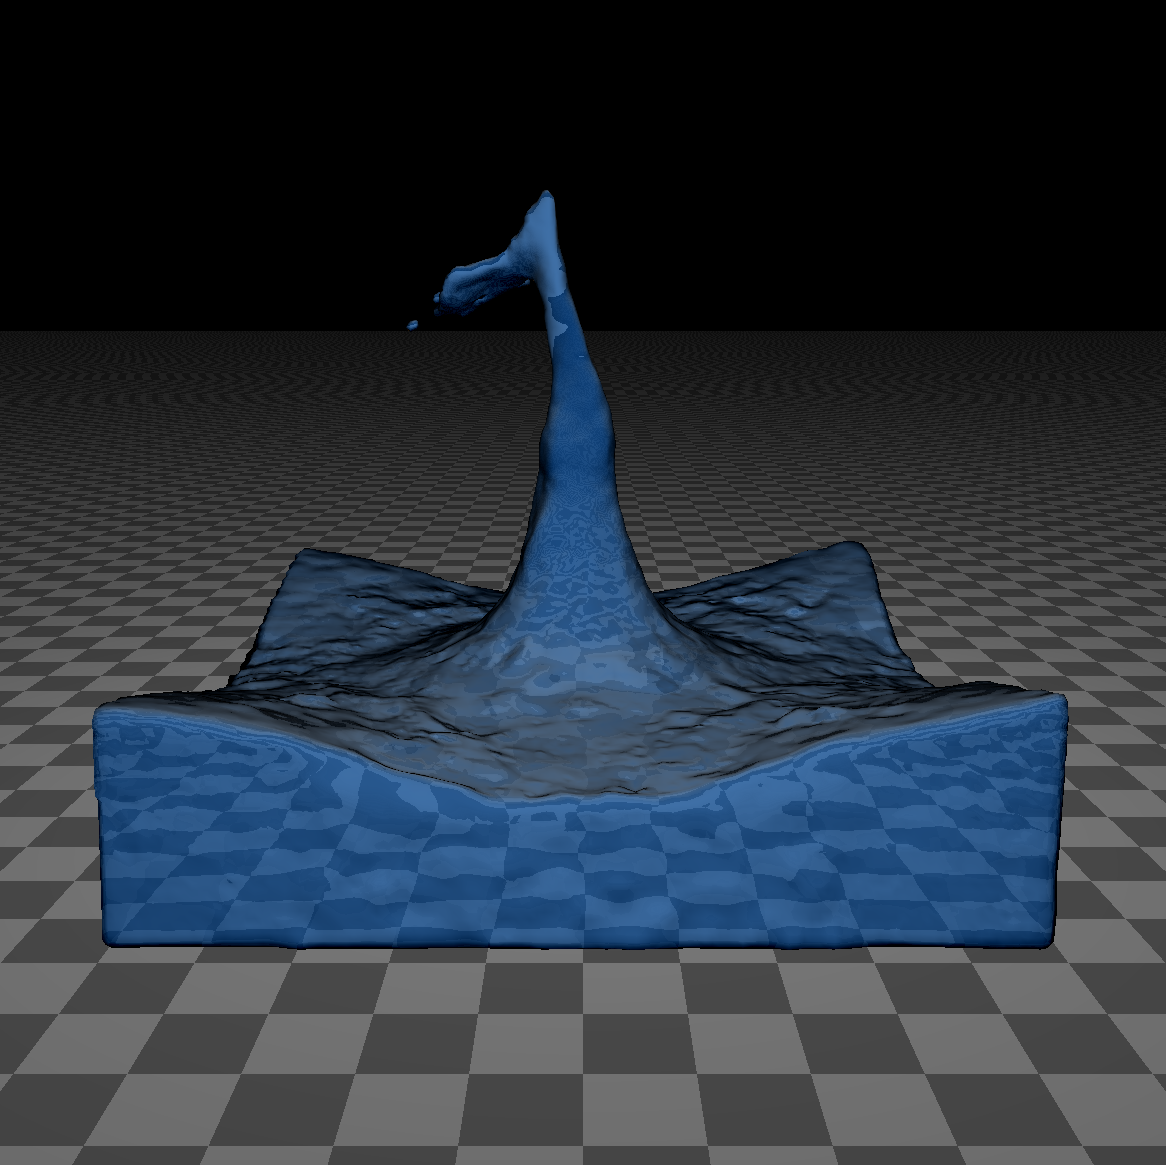
\includegraphics[width=5.7cm]{balldrop_cropped2/single2.png}
    \end{minipage}
    \begin{minipage}[t]{6.2cm}
        \centering
        \vspace{0pt}
        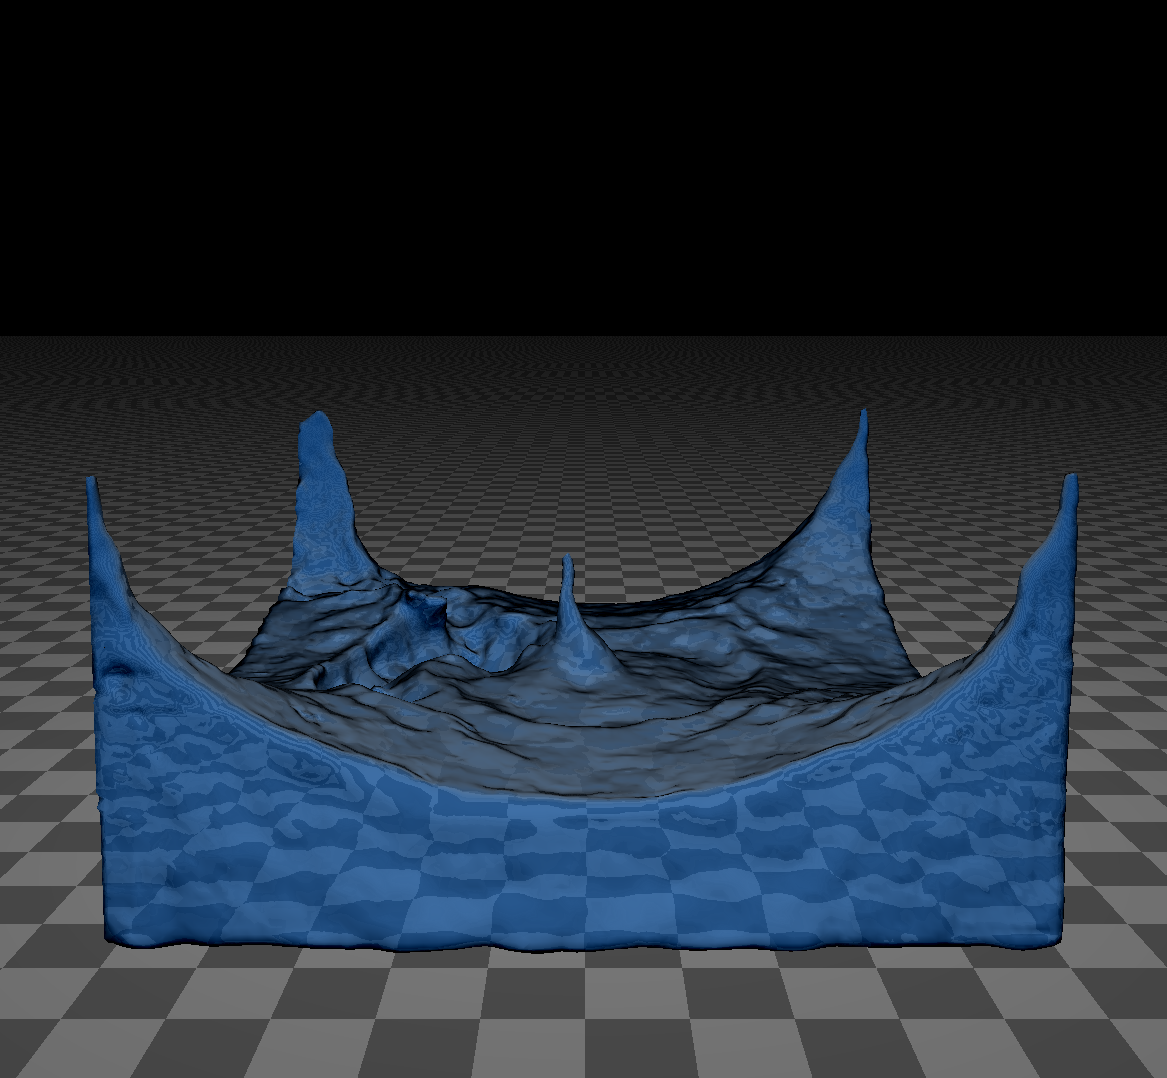
\includegraphics[width=5.7cm]{balldrop_cropped2/single3.png}
    \end{minipage}

    \caption{Ball drop. $50^3$ grid, $208k$ FLIP particles}
    \label{figure ball drop single}
\end{figure}

\newpage
\thispagestyle{empty}
\vspace*{-4cm}

\begin{figure}[H]
    \centering
    
    \begin{minipage}[t]{6.2cm}
        \centering
        \vspace{0pt}
        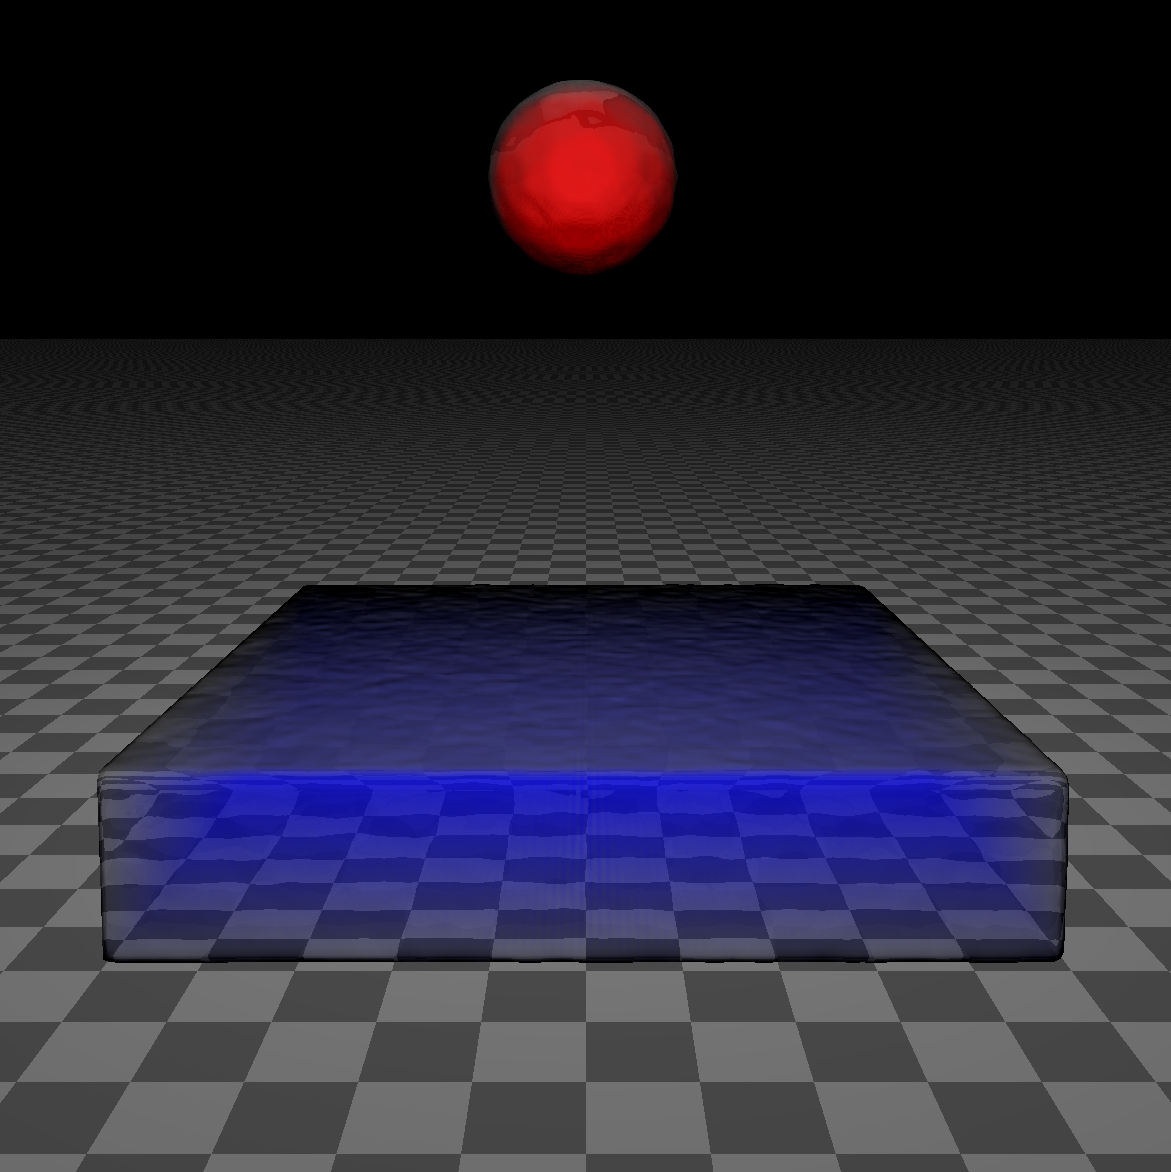
\includegraphics[width=5.7cm]{balldrop_cropped2/multi0.png}
    \end{minipage}
    \begin{minipage}[t]{6.2cm}
        \centering
        \vspace{0pt}
        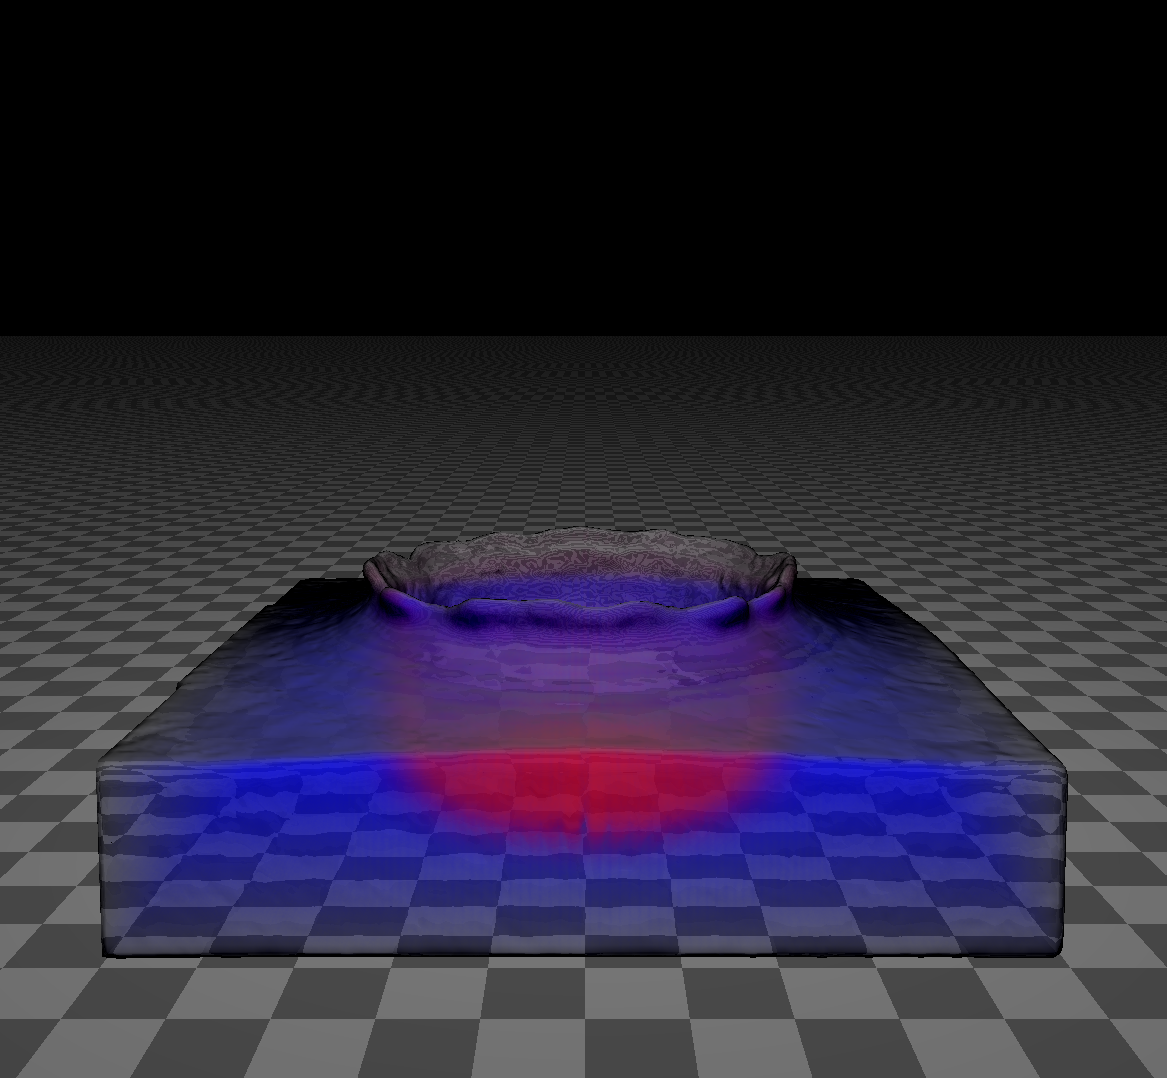
\includegraphics[width=5.7cm]{balldrop_cropped2/multi1.png}
    \end{minipage}

    \vspace{0.5cm}

    \begin{minipage}[t]{6.2cm}
        \centering
        \vspace{0pt}
        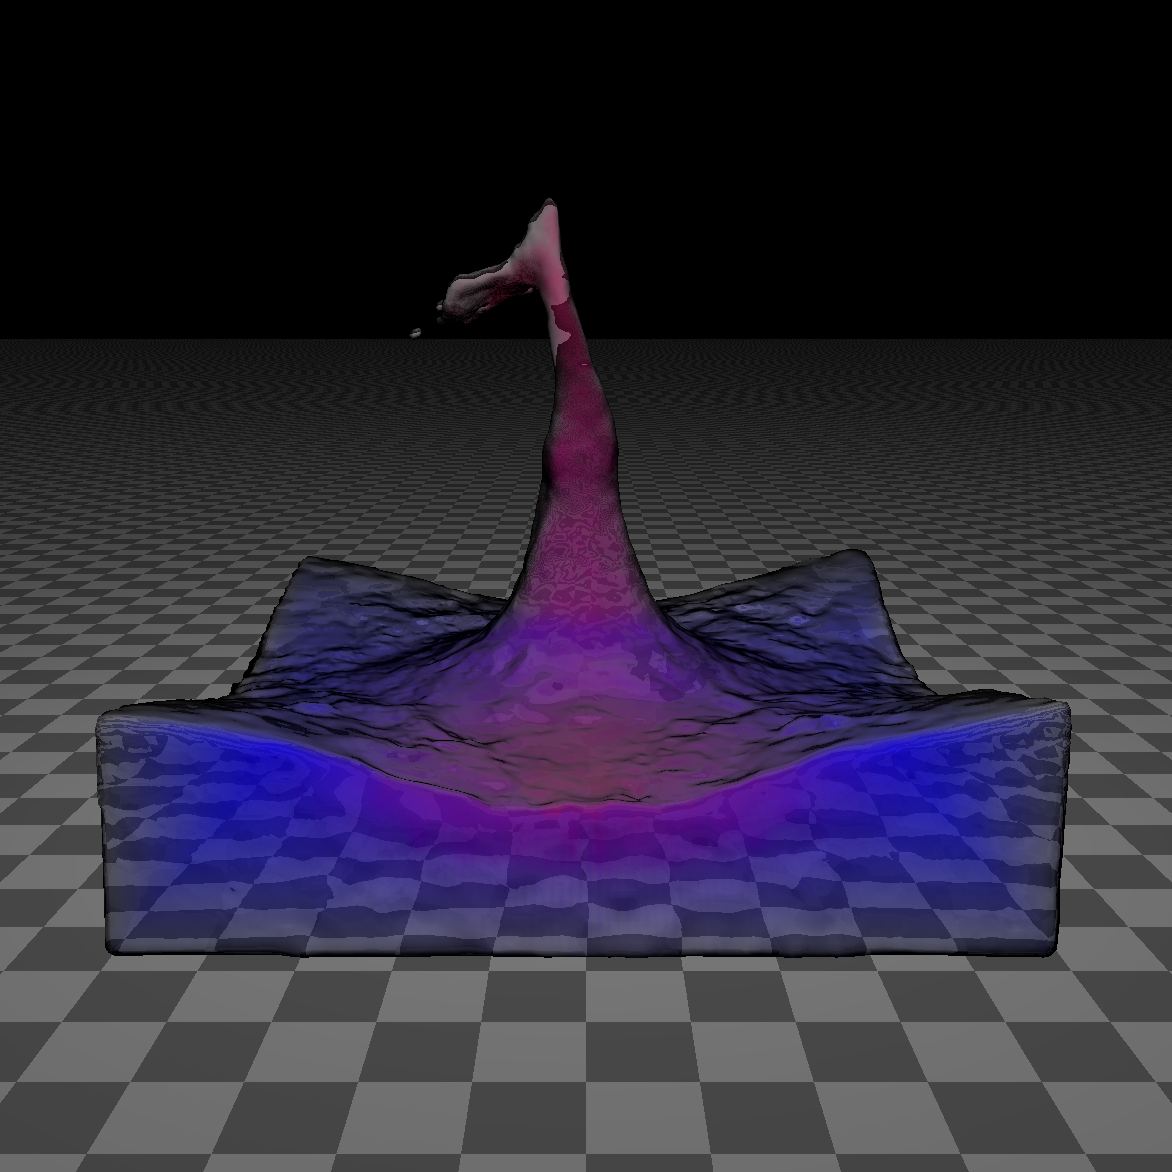
\includegraphics[width=5.7cm]{balldrop_cropped2/multi2.png}
    \end{minipage}
    \begin{minipage}[t]{6.2cm}
        \centering
        \vspace{0pt}
        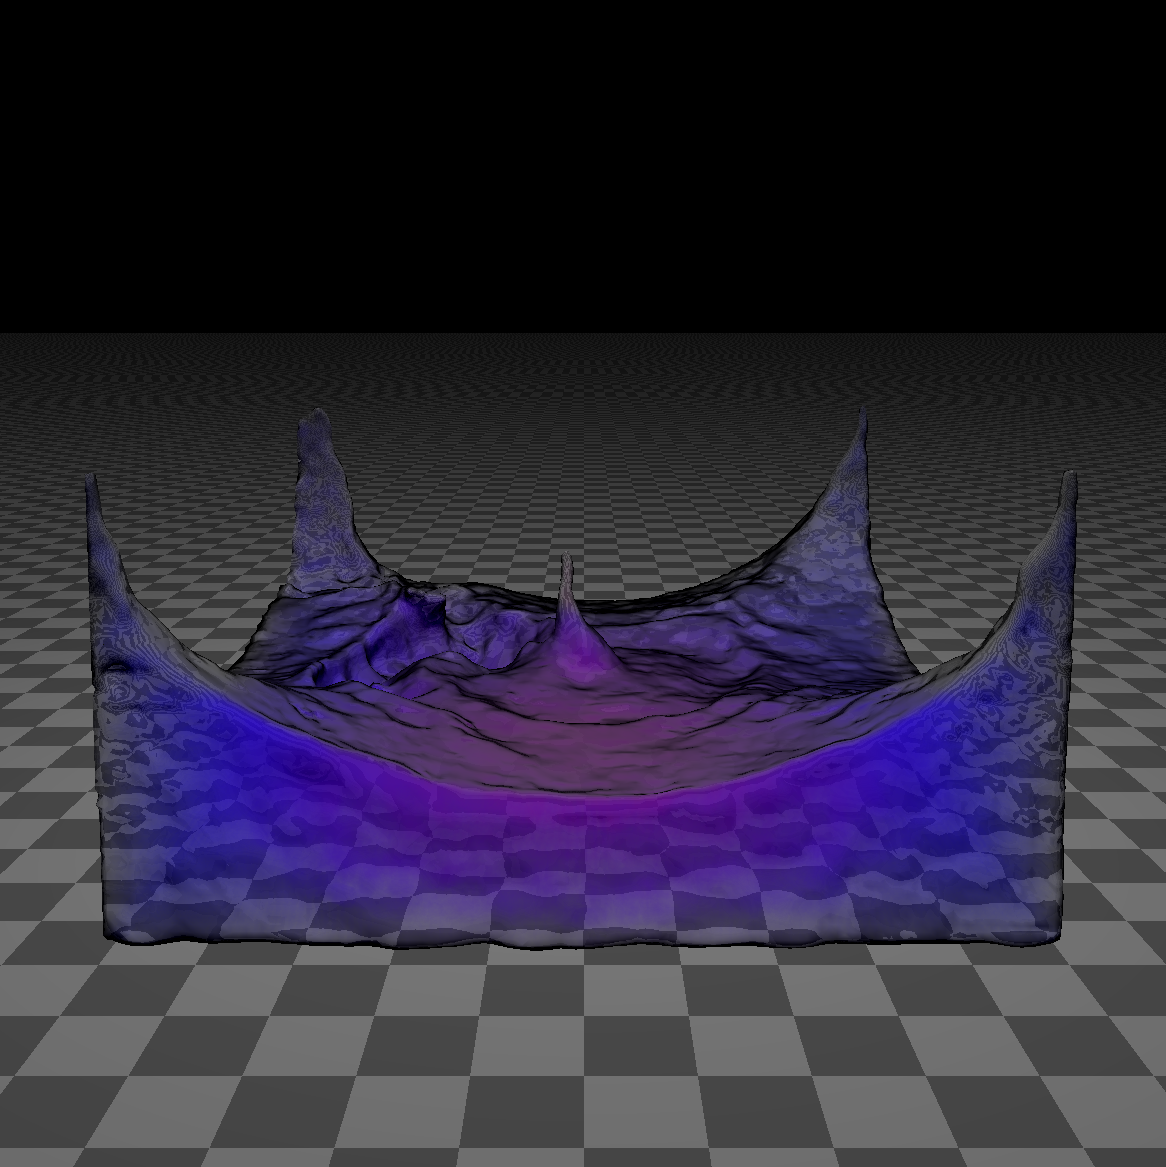
\includegraphics[width=5.7cm]{balldrop_cropped2/multi3.png}
    \end{minipage}

    \caption{Same simulation as figure \ref{figure ball drop single}, with 2 differently colored phases}
    \label{figure ball drop multi}
\end{figure}



\begin{figure}[H]
    \centering
    
    \begin{minipage}[t]{6.2cm}
        \centering
        \vspace{0pt}
        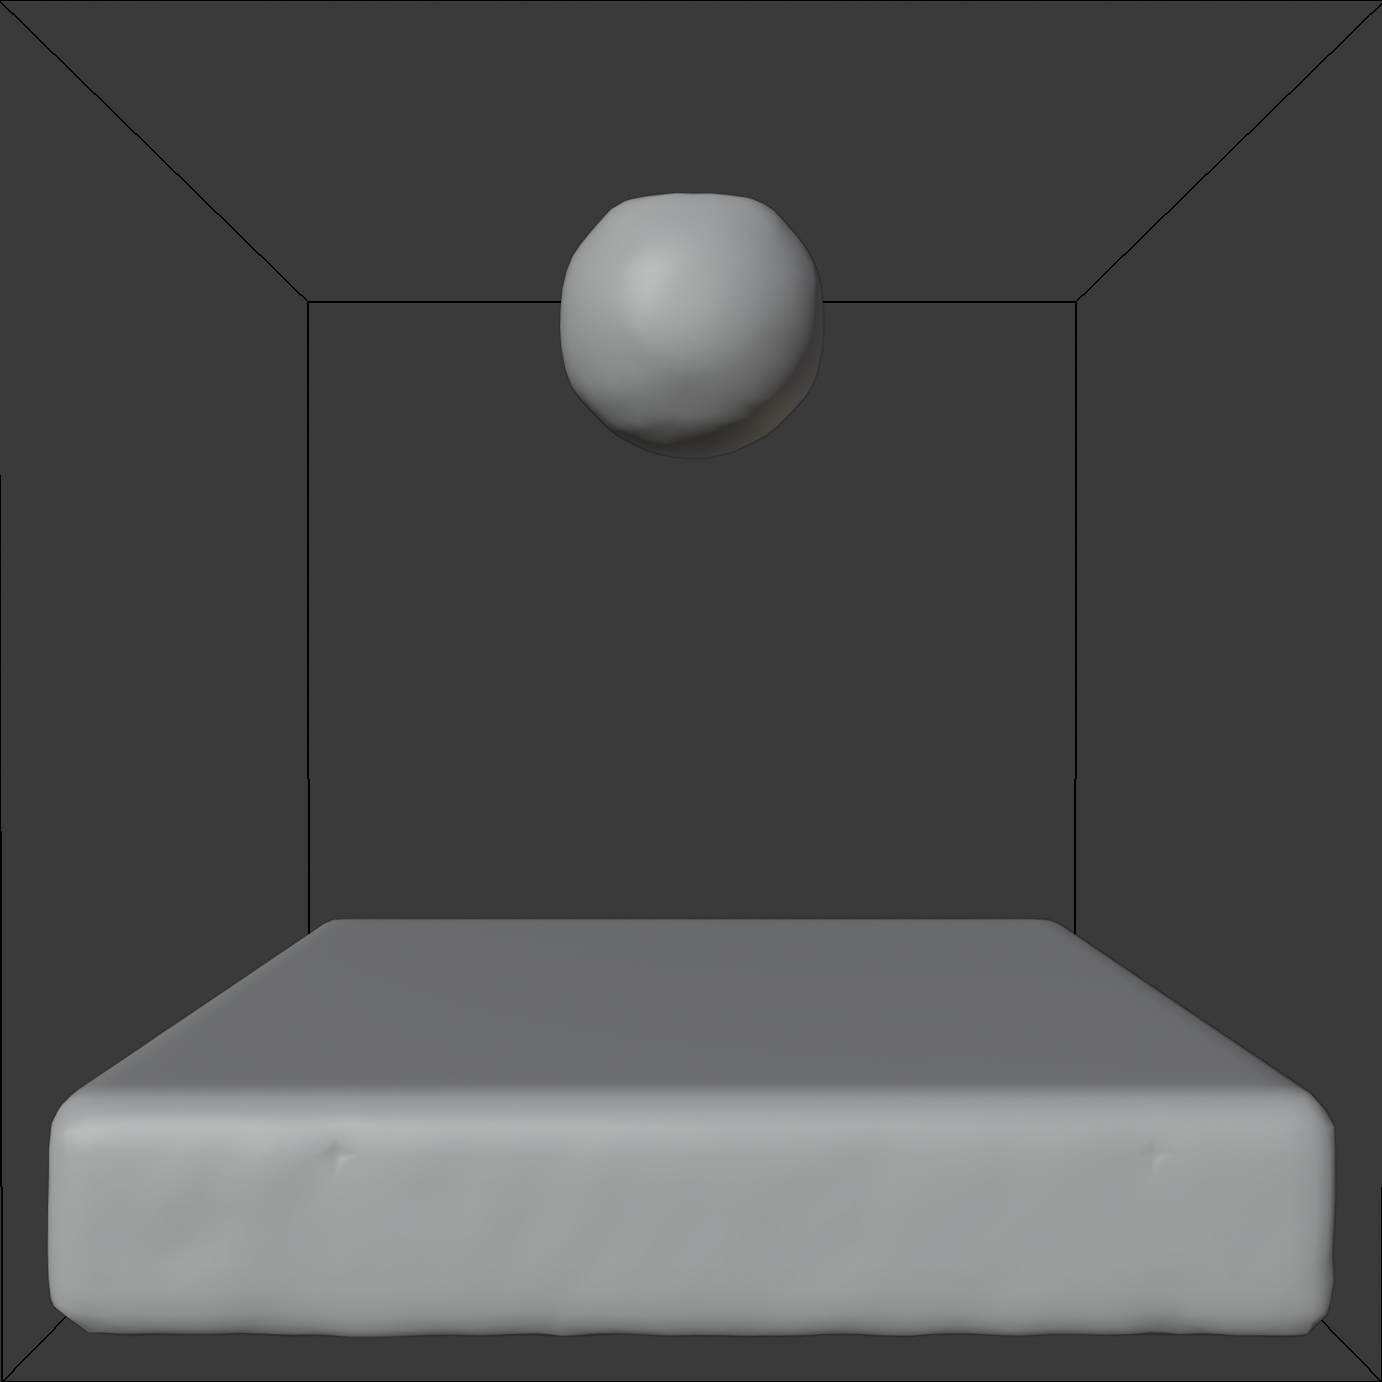
\includegraphics[width=5.7cm]{balldrop_cropped2/blender0.png}
    \end{minipage}
    \begin{minipage}[t]{6.2cm}
        \centering
        \vspace{0pt}
        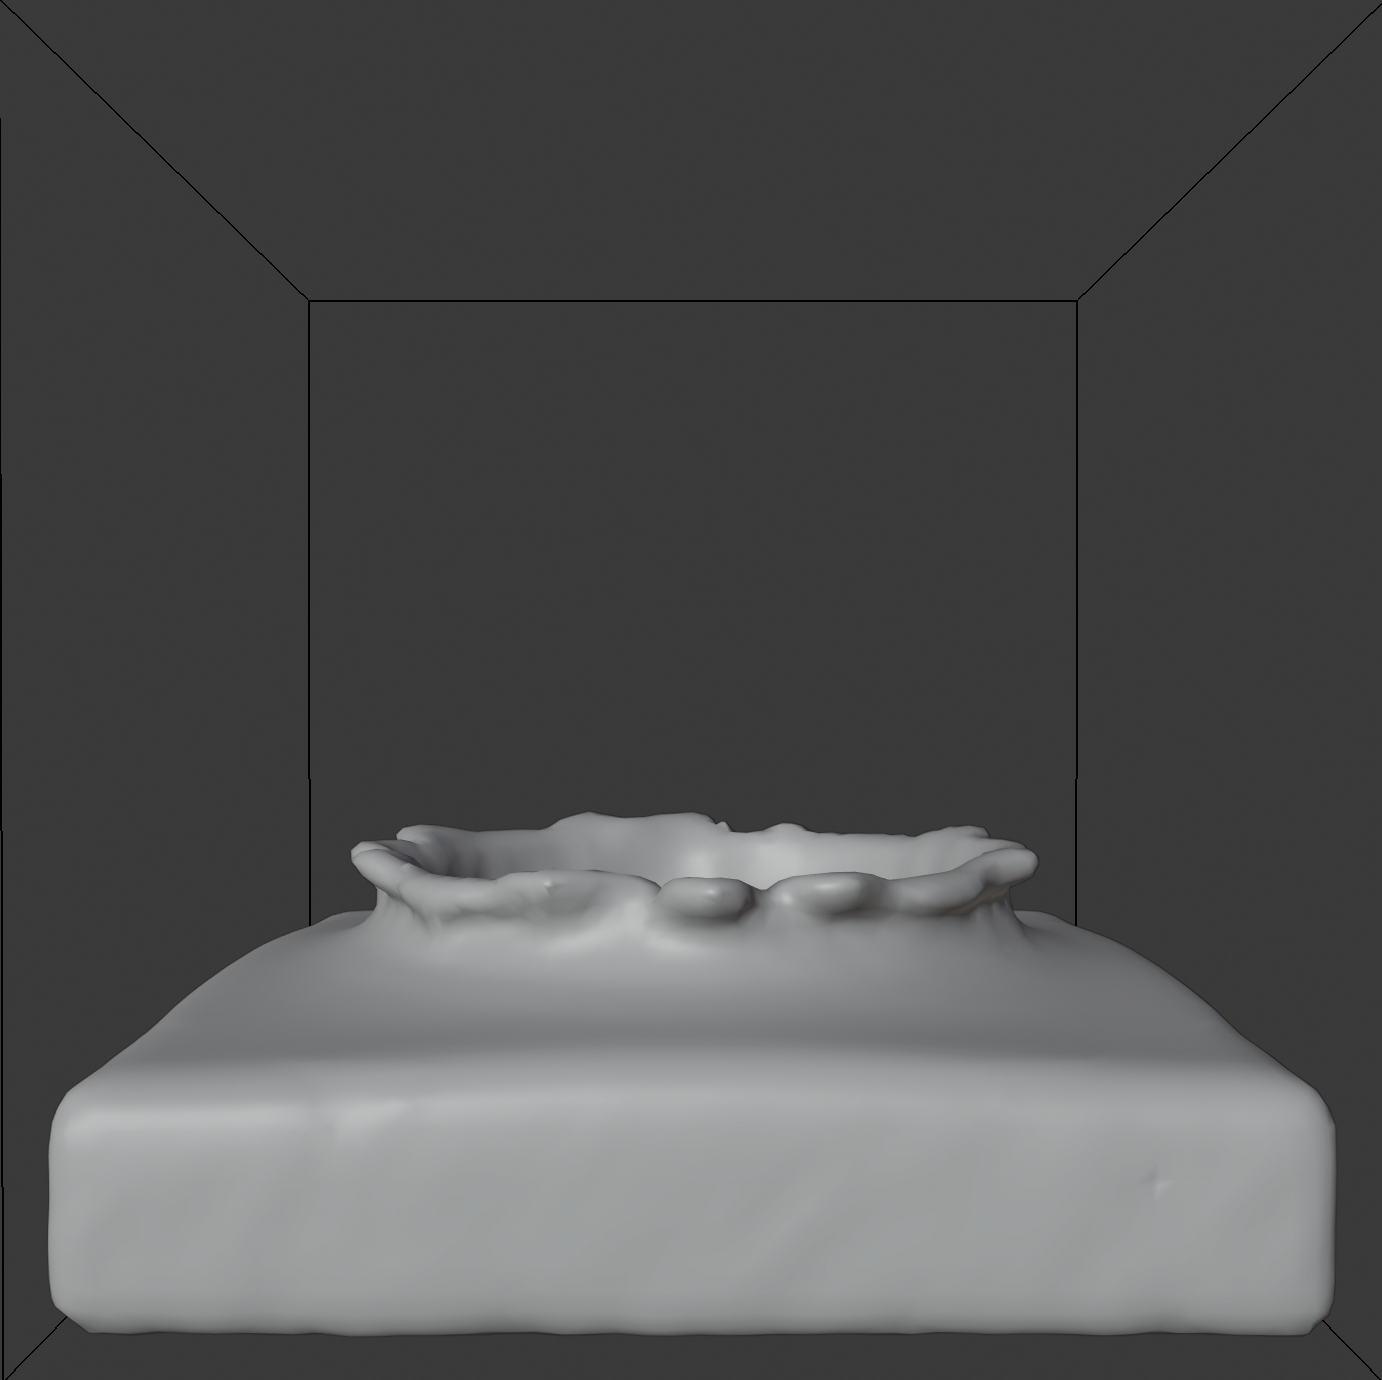
\includegraphics[width=5.7cm]{balldrop_cropped2/blender1.png}
    \end{minipage}

    \vspace{0.5cm}

    \begin{minipage}[t]{6.2cm}
        \centering
        \vspace{0pt}
        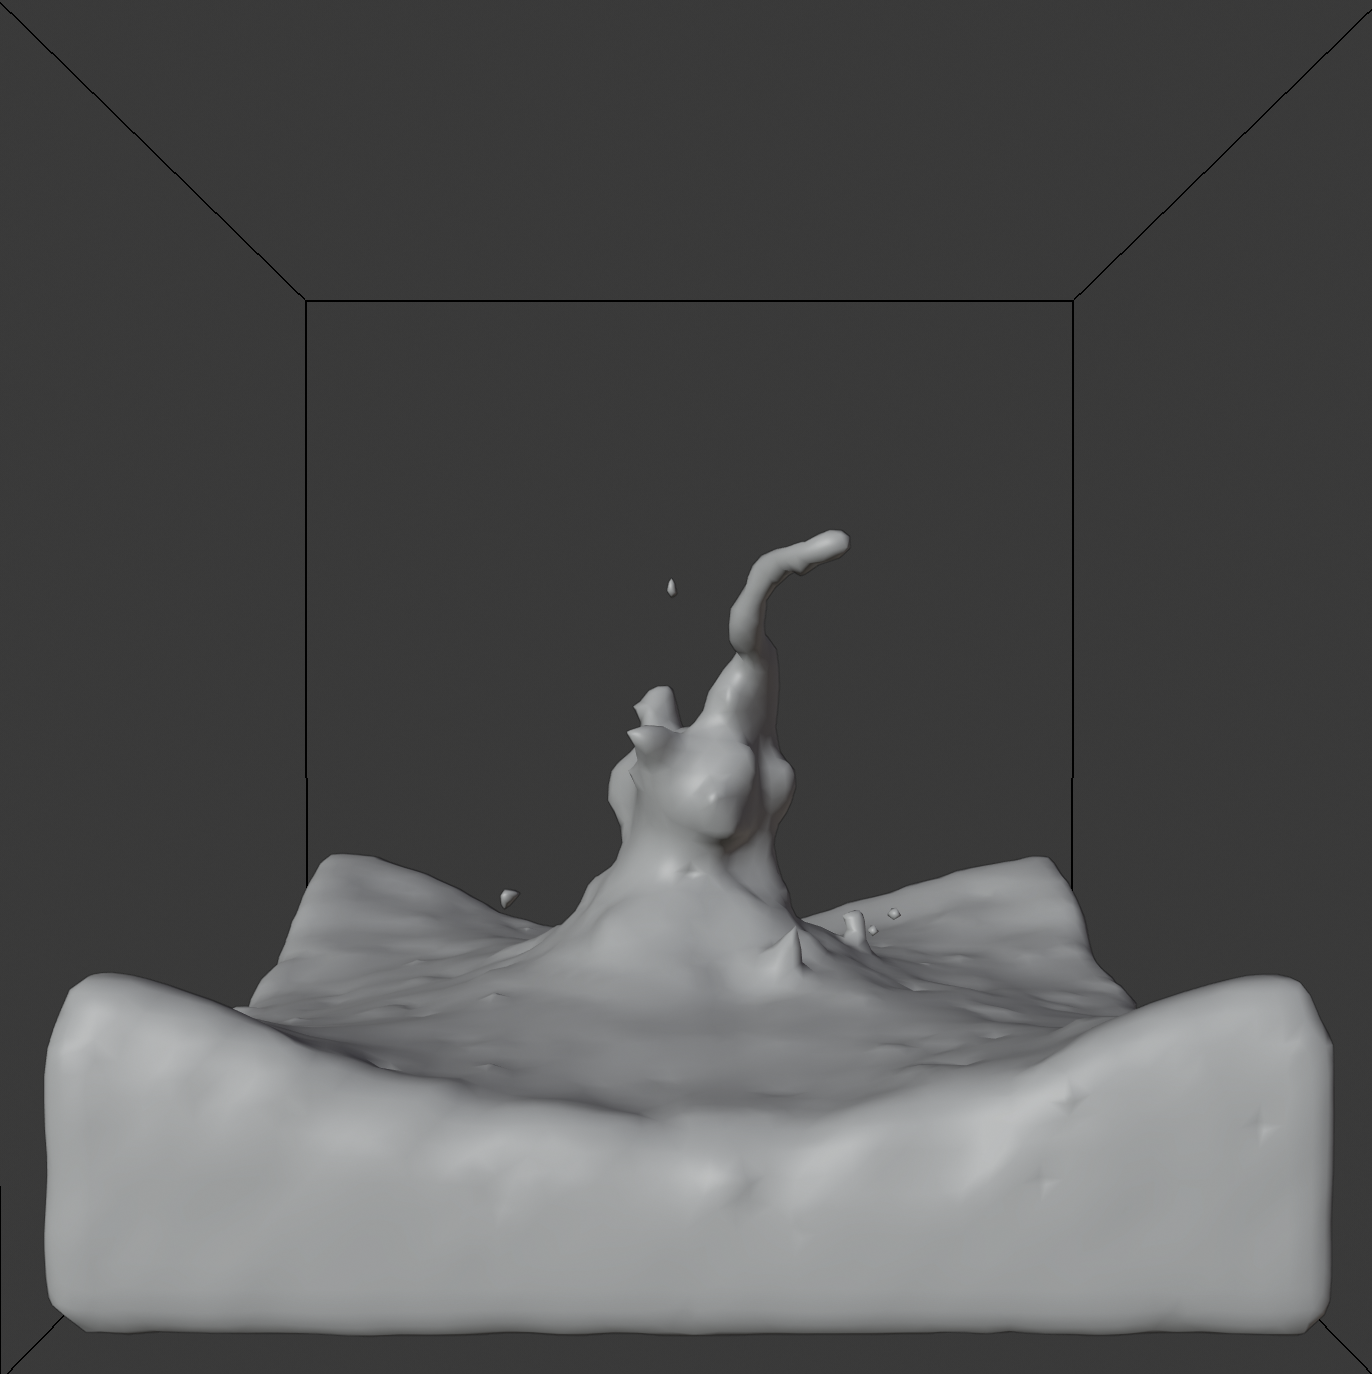
\includegraphics[width=5.7cm]{balldrop_cropped2/blender2.png}
    \end{minipage}
    \begin{minipage}[t]{6.2cm}
        \centering
        \vspace{0pt}
        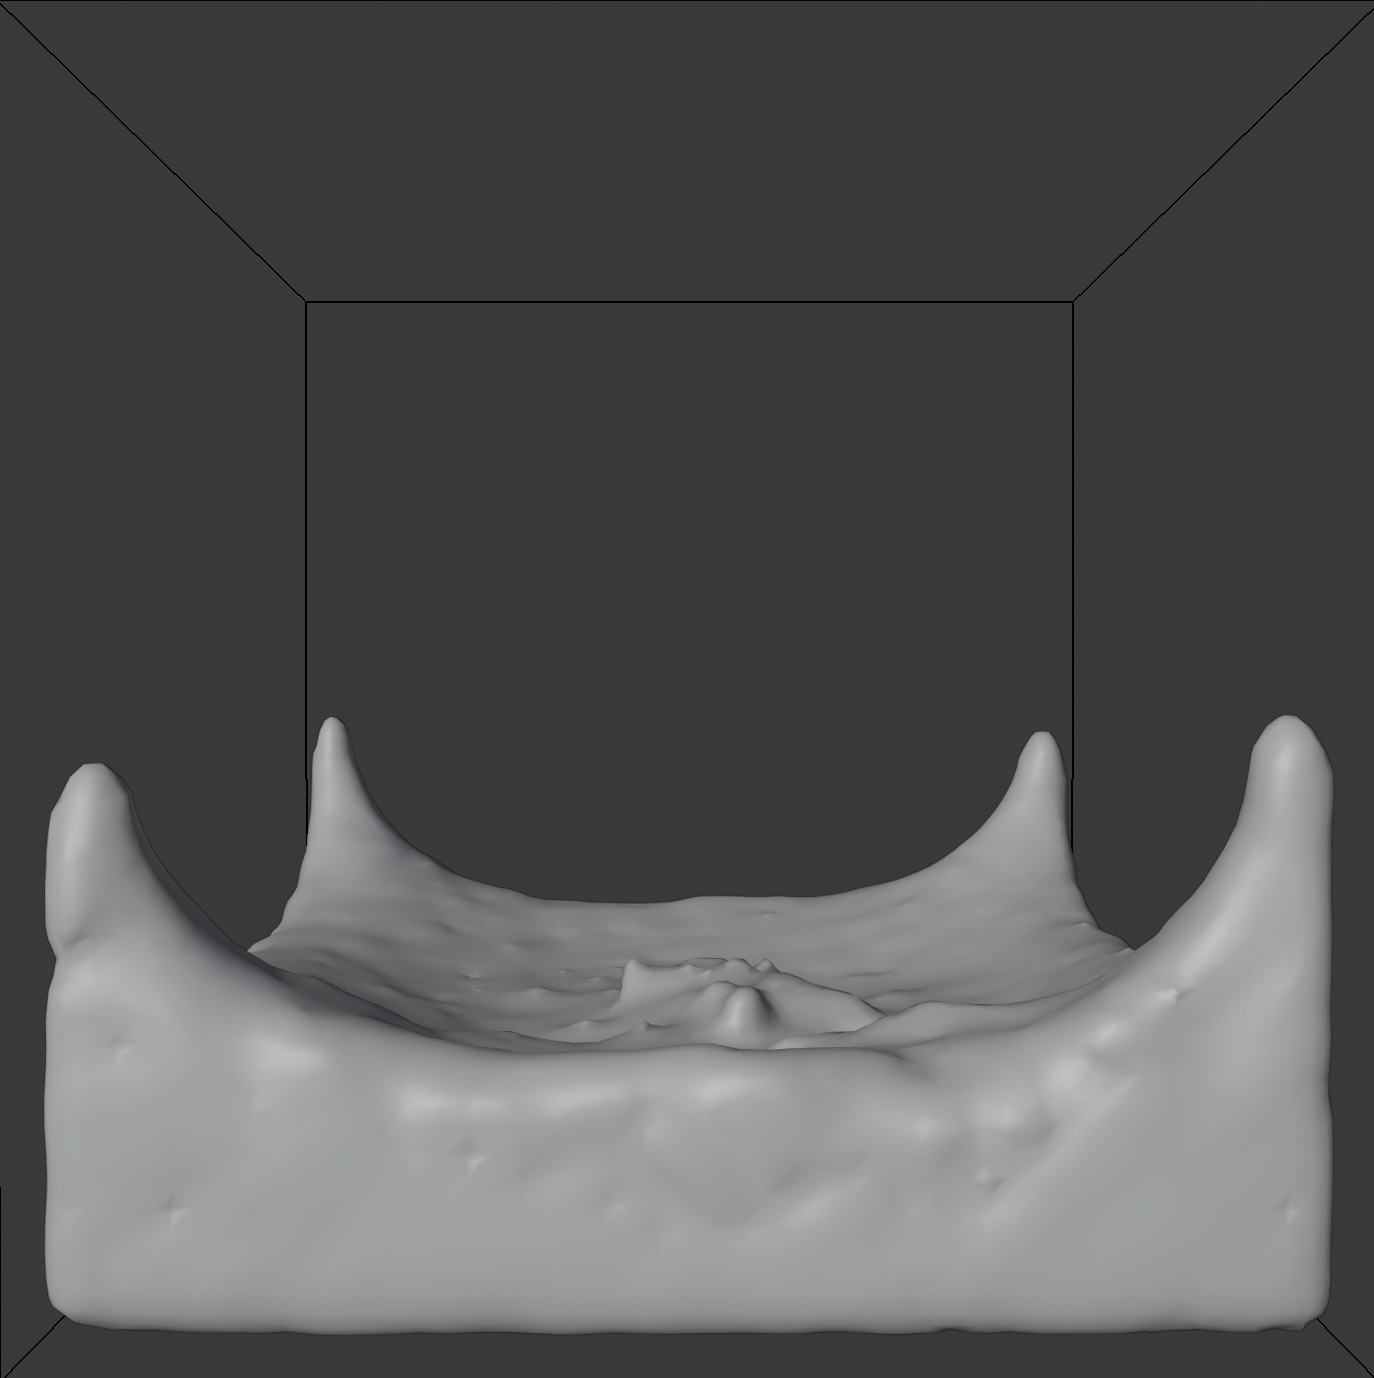
\includegraphics[width=5.7cm]{balldrop_cropped2/blender3.png}
    \end{minipage}

    \caption{Same simulation as figure \ref{figure ball drop single}, using a Blender add-on}
    \label{figure ball drop blender}
\end{figure}


%\addtolength{\topmargin}{1.1in}